\documentclass[conference]{IEEEtran}
\IEEEoverridecommandlockouts
% The preceding line is only needed to identify funding in the first footnote. If that is unneeded, please comment it out.
%Template version as of 6/27/2024

\usepackage{cite}
\usepackage{float}
\usepackage{amsmath,amssymb,amsfonts}
\usepackage{algorithmic}
\usepackage{graphicx}
\usepackage{textcomp}
\usepackage{xcolor}
\usepackage[brazilian]{babel}  % ou \usepackage[portuguese]{babel}
\usepackage[skip=10pt]{caption} % Ajusta o espaço para todas as legendas
\renewcommand{\tablename}{Tabela}

\def\BibTeX{{\rm B\kern-.05em{\sc i\kern-.025em b}\kern-.08em
    T\kern-.1667em\lower.7ex\hbox{E}\kern-.125emX}}
\begin{document}

\title{Análise Comparativa entre \textit{K-Means} e \textit{Robust Sparse K-Means} na Visualização de Padrões de Acidentes Ferroviários}

\author{
    \IEEEauthorblockN{Mateus Mendonça Monteiro\textsuperscript{1} and Cassio Machiaveli Oishi\textsuperscript{2}}
    \IEEEauthorblockA{
        \textit{Departamento de Matemática e Computação},\\
        \textit{Universidade Estadual Paulista}\\
        Presidente Prudente, Brasil\\
        mateus.monteiro@unesp.br, cassio.oishi@unesp.br
    }
}

\maketitle

\begin{abstract}
Este trabalho apresenta uma análise comparativa entre as técnicas de \textit{clustering} \textit{K-means} tradicional e \textit{Robust Sparse K-means} aplicadas à análise de acidentes ferroviários no Brasil, utilizando dados disponibilizados publicamente pela Agência Nacional de Transportes Terrestres (ANTT) através do portal Dados Abertos, compreendendo uma amostra do período entre 2020 e 2024. A pesquisa desenvolveu uma metodologia que combina técnicas robustas de \textit{clustering} com visualizações geoespaciais interativas para identificar padrões nos acidentes ferroviários.
\end{abstract}

\begin{IEEEkeywords}
Visualização de Dados, K-Means, Robust Sparse K-Means, Análise de Acidentes Ferroviários, Clusterização, ANTT, Técnicas de Visualização
\end{IEEEkeywords}

\section{Introdução}
\subsection{Contextualização do Problema}

A Agência Nacional de Transportes Terrestres (ANTT) mantém registros detalhados destes acidentes através do Relatório de Acompanhamento de Acidentes Ferroviários (RAAF), atualizado em 2025, gerando um volume considerável de dados que, embora rico em informações, apresenta desafios significativos para análise e interpretação. A complexidade destes dados deriva não apenas de seu volume, mas também da diversidade de variáveis envolvidas, incluindo causas diretas e contributivas, impactos financeiros, características operacionais e condições geográficas. Estudos recentes, como o trabalho de Meng et al. \cite{b6}, demonstram que a aplicação de técnicas avançadas de análise de dados pode fornecer \textit{insights} valiosos sobre os fatores críticos relacionados a acidentes ferroviários, contribuindo significativamente para o desenvolvimento de mecanismos de alerta precoce e prevenção de ocorrências.

\section{Trabalhos Relacionados}

A análise de acidentes ferroviários tem sido objeto de diversos estudos que empregam técnicas avançadas de análise de dados. Meng et al. \cite{b6} propuseram uma abordagem baseada em \textit{ensemble learning} para previsão de acidentes ferroviários, alcançando resultados significativos na identificação de fatores de risco críticos relacionados a descarrilhamentos e colisões. Seu trabalho demonstrou a eficácia de técnicas de aprendizado de máquina na análise de dados ferroviários, obtendo métricas de desempenho expressivas (\textit{Accuracy}: 0.879, \textit{Precision}: 0.879, \textit{Recall}: 0.883 e \textit{F1-score}: 0.881).

A abordagem desse estudo se diferencia ao focar na análise comparativa entre técnicas de \textit{clustering}, especificamente o \textit{K-means} tradicional e o \textit{Robust Sparse K-means}, com ênfase na visualização geoespacial dos padrões de acidentes. Além disso, este busca identificar padrões espaciais e temporais que possam informar estratégias de prevenção e gestão de segurança.

\subsection{Motivação}
A motivação principal deste trabalho emerge do potencial em desenvolver metodologias avançadas para análise e compreensão de padrões em acidentes ferroviários, visando contribuir com as análises já realizadas pela ANTT. O estudo propõe complementar os métodos existentes através da integração de técnicas de clusterização robusta com visualizações geoespaciais interativas, oferecendo novas perspectivas para a análise de segurança ferroviária no Brasil.

Esta abordagem metodológica pode complementar as ferramentas existentes da ANTT, fornecendo uma perspectiva adicional para estudos e análises de acidentes ferroviários pela agência.

A escolha de combinar técnicas avançadas de clusterização com visualizações interativas é motivada pela necessidade de:
\begin{itemize}
\item Identificar padrões espaciais não evidentes em análises convencionais.
\item Determinar automaticamente a relevância de diferentes variáveis na caracterização de acidentes.
\item Facilitar a compreensão de padrões complexos através de visualizações interativas.
\end{itemize}

\subsection{Objetivos}
O objetivo principal deste trabalho é desenvolver e avaliar uma abordagem comparativa entre o \textit{K-Means} tradicional e o \textit{Robust Sparse K-Means} para análise e visualização de padrões em acidentes ferroviários. Especificamente, busca-se:

1. Implementar uma metodologia robusta para processamento e análise de dados de acidentes ferroviários, incluindo enriquecimento geográfico através de geocodificação.

2. Desenvolver visualizações interativas que permitam a exploração efetiva de padrões espaciais em acidentes ferroviários.

3. Comparar e avaliar a eficácia do \textit{K-Means} tradicional e do \textit{Robust Sparse K-Means} na identificação de padrões significativos.

4. Propor métricas objetivas para avaliação da qualidade dos \textit{clusters} e das visualizações resultantes.

\subsection{Contribuições}
Este trabalho apresenta as seguintes contribuições principais:

1. \textbf{Metodológicas:}
   - Desenvolvimento de uma abordagem integrada para análise de acidentes ferroviários.
   - Adaptação do \textit{Robust Sparse K-Means} para dados de transportes.
   - Proposição de métricas específicas para avaliação de \textit{clusters} em dados ferroviários.

2. \textbf{Técnicas:}
   - Implementação de um pipeline completo de processamento e análise.
   - Desenvolvimento de visualizações interativas customizadas.
   - Enriquecimento geográfico automatizado dos dados.

3. \textbf{Práticas:}
   - Identificação de padrões relevantes para segurança ferroviária.
   - Geração de \textit{insights} acionáveis para gestores.
   - Criação de uma base metodológica para análises futuras.

\section{Base de Dados}

\subsection{Descrição dos Dados}
Este trabalho utiliza dados provenientes do Relatório de Acompanhamento de Acidentes Ferroviários (RAAF) da Agência Nacional de Transportes Terrestres (ANTT). O conjunto de dados abrange um período de 20 anos, compreendendo registros de acidentes ferroviários ocorridos no Brasil entre 2020 e 2024. A base de dados encontra-se disponível publicamente através do Portal de Dados Abertos da ANTT \cite{b1}, demonstrando o compromisso da agência com a transparência e o acesso à informação.

O conjunto completo apresenta uma estrutura multidimensional, incorporando 32 atributos que descrevem diferentes aspectos de cada ocorrência. Estes atributos podem ser cate gorizados em cinco dimensões principais: informações temporais, dados geográficos, características do acidente, aspectos operacionais e impactos resultantes.

\subsection{Informações Temporais e Geográficas}
As informações temporais são registradas com granularidade até o nível de hora, permitindo análises detalhadas de padrões temporais. Cada registro contém:

\begin{itemize}
\item Data da ocorrência (Data\_Ocorrencia): formato YYYY-MM-DD.
\item Hora do acidente (Hora\_Ocorrencia): formato HH:MM.
\item Período do dia: derivado da hora da ocorrência.
\end{itemize}

A localização geográfica é especificada através de múltiplos níveis de granularidade:
\begin{itemize}
\item Unidade Federativa (UF).
\item Município.
\item Linha férrea específica.
\item Quilometragem inicial e final do trecho.
\item Estações anterior e posterior ao local do acidente.
\item Indicador de perímetro urbano.
\end{itemize}

\subsection{Características do Acidente}
Cada ocorrência é caracterizada por um conjunto detalhado de atributos que descrevem a natureza e as circunstâncias do acidente:

\begin{itemize}
\item Gravidade do acidente.
\item Causa direta: fator principal que ocasionou o acidente.
\item Causa contributiva: fatores secundários que influenciaram a ocorrência.
\item Natureza do acidente: classificação do tipo de ocorrência.
\item Presença de passagem em nível (PN).
\item Envolvimento de outras ferrovias.
\end{itemize}

\subsection{Aspectos Operacionais}
Os dados operacionais fornecem contexto sobre as condições e características do serviço ferroviário no momento do acidente:

\begin{itemize}
\item Concessionária responsável.
\item Serviço de transporte.
\item Prefixo e número do trem.
\item Tipo de carga transportada.
\item Utilização de \textit{Double Stack}.
\item Equipagem envolvida.
\end{itemize}

\subsection{Impactos}
O registro dos impactos abrange tanto aspectos humanos quanto operacionais e financeiros:

\begin{itemize}
\item Número de feridos.
\item Número de óbitos.
\item Tempo de interrupção da via.
\item Prejuízo financeiro (em Reais).
\end{itemize}

\subsection{Limitações e Qualidade dos Dados}
Apesar da riqueza de informações, o conjunto de dados apresenta algumas limitações importantes:

\begin{itemize}
\item Ausência de coordenadas geográficas precisas.
\item Inconsistências no formato de registros temporais.
\item Valores ausentes em campos críticos.
\item Variações na padronização de nomenclaturas.
\item Potencial subnotificação de acidentes menores.
\end{itemize}

\section{Pré-processamento e Enriquecimento dos Dados}

\subsection{Enriquecimento Geográfico}
O enriquecimento geográfico foi realizado através de um processo automatizado utilizando a API Google \textit{Geocoding} \cite{b5}:

\begin{enumerate}
\item Construção de \textit{strings} de localização combinando Município, UF e País.
\item Requisições à API para obtenção de coordenadas.
\item Validação das coordenadas retornadas.
\item Armazenamento de latitude e longitude.
\end{enumerate}

O processo de geocodificação seguiu o algoritmo:

\begin{algorithm}
\caption{Processo de Geocodificação}
\begin{algorithmic}[1]
\STATE Criar dicionário para armazenar coordenadas já conhecidas
\FORALL{acidente na base de dados}
    \IF{acidente já possui coordenadas}
        \STATE Armazenar no dicionário
        \STATE Continuar para próximo registro
    \ENDIF
    \IF{município já tem coordenadas no dicionário}
        \STATE Usar coordenadas armazenadas
    \ELSE
        \STATE Buscar coordenadas na Google Geocoding API
        \IF{coordenadas encontradas}
            \STATE Salvar no registro atual
            \STATE Armazenar no dicionário para uso futuro
        \ENDIF
        \STATE Aguardar brevemente antes da próxima busca
    \ENDIF
\ENDFOR
\STATE Salvar base de dados enriquecida
\end{algorithmic}
\end{algorithm}

\subsection{Tratamento de Dados}
O tratamento de dados envolveu múltiplas etapas de limpeza e padronização:

\begin{enumerate}
\item \textbf{Padronização de Formatos}:
   \begin{itemize}
   \item Conversão de datas para formato ISO.
   \item Normalização de valores monetários.
   \item Padronização de coordenadas geográficas.
   \end{itemize}

\item \textbf{Tratamento de Valores Ausentes}:
   \begin{itemize}
   \item Imputação de valores faltantes.
   \item Remoção de registros incompletos.
   \item Documentação de decisões de tratamento.
   \end{itemize}

\item \textbf{Normalização de Variáveis}:
   \begin{itemize}
   \item Escalonamento de variáveis numéricas.
   \item Codificação de variáveis categóricas.
   \item Transformação de variáveis temporais.
   \end{itemize}
\end{enumerate}

\section{Metodologia}

\subsection{Visão Geral da Abordagem}
Este trabalho propõe uma abordagem integrada para análise e visualização de padrões em acidentes ferroviários, combinando técnicas avançadas de \textit{clustering} com visualizações interativas. A metodologia desenvolvida fundamenta-se em três pilares principais: análise espacial, identificação de padrões temporais e visualização interativa de dados.

Nossa abordagem se diferencia das análises tradicionais ao incorporar técnicas robustas de \textit{clustering} que consideram automaticamente a relevância das variáveis, permitindo uma compreensão mais profunda dos padrões de acidentes. 

\subsection{Arquitetura do Sistema}

\subsubsection{Componentes Principais}
O sistema foi desenvolvido seguindo uma arquitetura modular, composta por quatro componentes principais :

1. \textbf{Módulo de Processamento de Dados:}
   - Responsável pela limpeza e preparação dos dados.
   - Implementa o enriquecimento geográfico.
   - Gerencia a normalização e transformação de variáveis.

2. \textbf{Módulo de Análise:}
   - Implementa os algoritmos de \textit{clustering}.
   - Executa análises estatísticas.
   - Calcula métricas de avaliação.

3. \textbf{Módulo de Visualização:}
   - Gera visualizações interativas.
   - Gerencia a interação com usuário.
   - Implementa diferentes tipos de gráficos e mapas.

4. \textbf{Interface do Usuário:}
   - Desenvolvida com \textit{Streamlit}.
   - Fornece controles interativos.
   - Apresenta resultados dinâmicos.

\subsubsection{Fluxo de Processamento}
O fluxo de processamento segue uma sequência lógica de operações:

1. \textbf{Ingestão de Dados:}
\begin{equation}
D_{raw} \xrightarrow{\text{leitura}} D_{input}
\end{equation}

2. \textbf{Pré-processamento:}
\begin{equation}
D_{input} \xrightarrow{\text{normalização}} D_{processed}
\end{equation}

3. \textbf{Análise:}
\begin{equation}
D_{processed} \xrightarrow{\text{clustering}} D_{analyzed}
\end{equation}

4. \textbf{Visualização:}
\begin{equation}
D_{analyzed} \xrightarrow{\text{renderização}} V_{output}
\end{equation}

\subsubsection{Tecnologias Utilizadas}
O sistema foi implementado utilizando um conjunto moderno de tecnologias de código aberto:

\begin{itemize}
\item \textit{Python} 3.10 como linguagem principal.
\item Pandas para manipulação de dados.
\item \textit{Scikit-learn} para implementação dos algoritmos.
\item \textit{Plotly} para visualizações interativas.
\item \textit{Streamlit} para interface web.
\end{itemize}

\subsection{Técnicas de Clustering}

\subsubsection{K-Means Tradicional}
O algoritmo \textit{K-means tradicional} \cite{b3} é implementado como baseline para comparação, seguindo a formulação clássica:

\begin{equation}
\min_{\{C_k\}_{k=1}^K} \sum_{k=1}^K \sum_{x_i \in C_k} ||x_i - \mu_k||^2
\end{equation}

onde $C_k$ representa o k-ésimo \textit{cluster} e $\mu_k$ seu centróide.

\subsubsection{Determinação do Número Ótimo de Clusters}
O número ótimo de \textit{clusters} é determinado através do método do cotovelo \cite{b4}, analisando a variação da inércia:

\begin{equation}
\text{\textit{Inertia}}(k) = \sum_{i=1}^n \min_{\mu_j \in C} ||x_i - \mu_j||^2
\end{equation}

O ponto de inflexão na curva de inércia indica o número ideal de \textit{clusters}.

\subsubsection{Robust Sparse K-Means com LASSO}
O \textit{Robust Sparse K-means} \cite{b2} incorpora regularização LASSO para seleção automática de características:

\begin{equation}
\min_{\{C_k\}_{k=1}^K, w} \sum_{k=1}^K \sum_{x_i \in C_k} \sum_{j=1}^p w_j||x_{ij} - \mu_{kj}||^2 + \lambda||w||_1
\end{equation}

sujeito a:
\begin{equation}
\sum_{j=1}^p w_j = 1, w_j \geq 0
\end{equation}

\section{Sistema de Visualização e Análise}

O desenvolvimento deste trabalho resultou em um sistema interativo completo de visualização e análise de acidentes ferroviários, implementado utilizando \textit{Streamlit} e \textit{Python}. O sistema integra múltiplas perspectivas de análise, permitindo uma compreensão abrangente dos padrões de acidentes.

\subsection{Interface e Funcionalidades}

A interface do sistema foi projetada para facilitar a exploração interativa dos dados, oferecendo diferentes níveis de análise:

\begin{figure}[!htb]
    \centering
    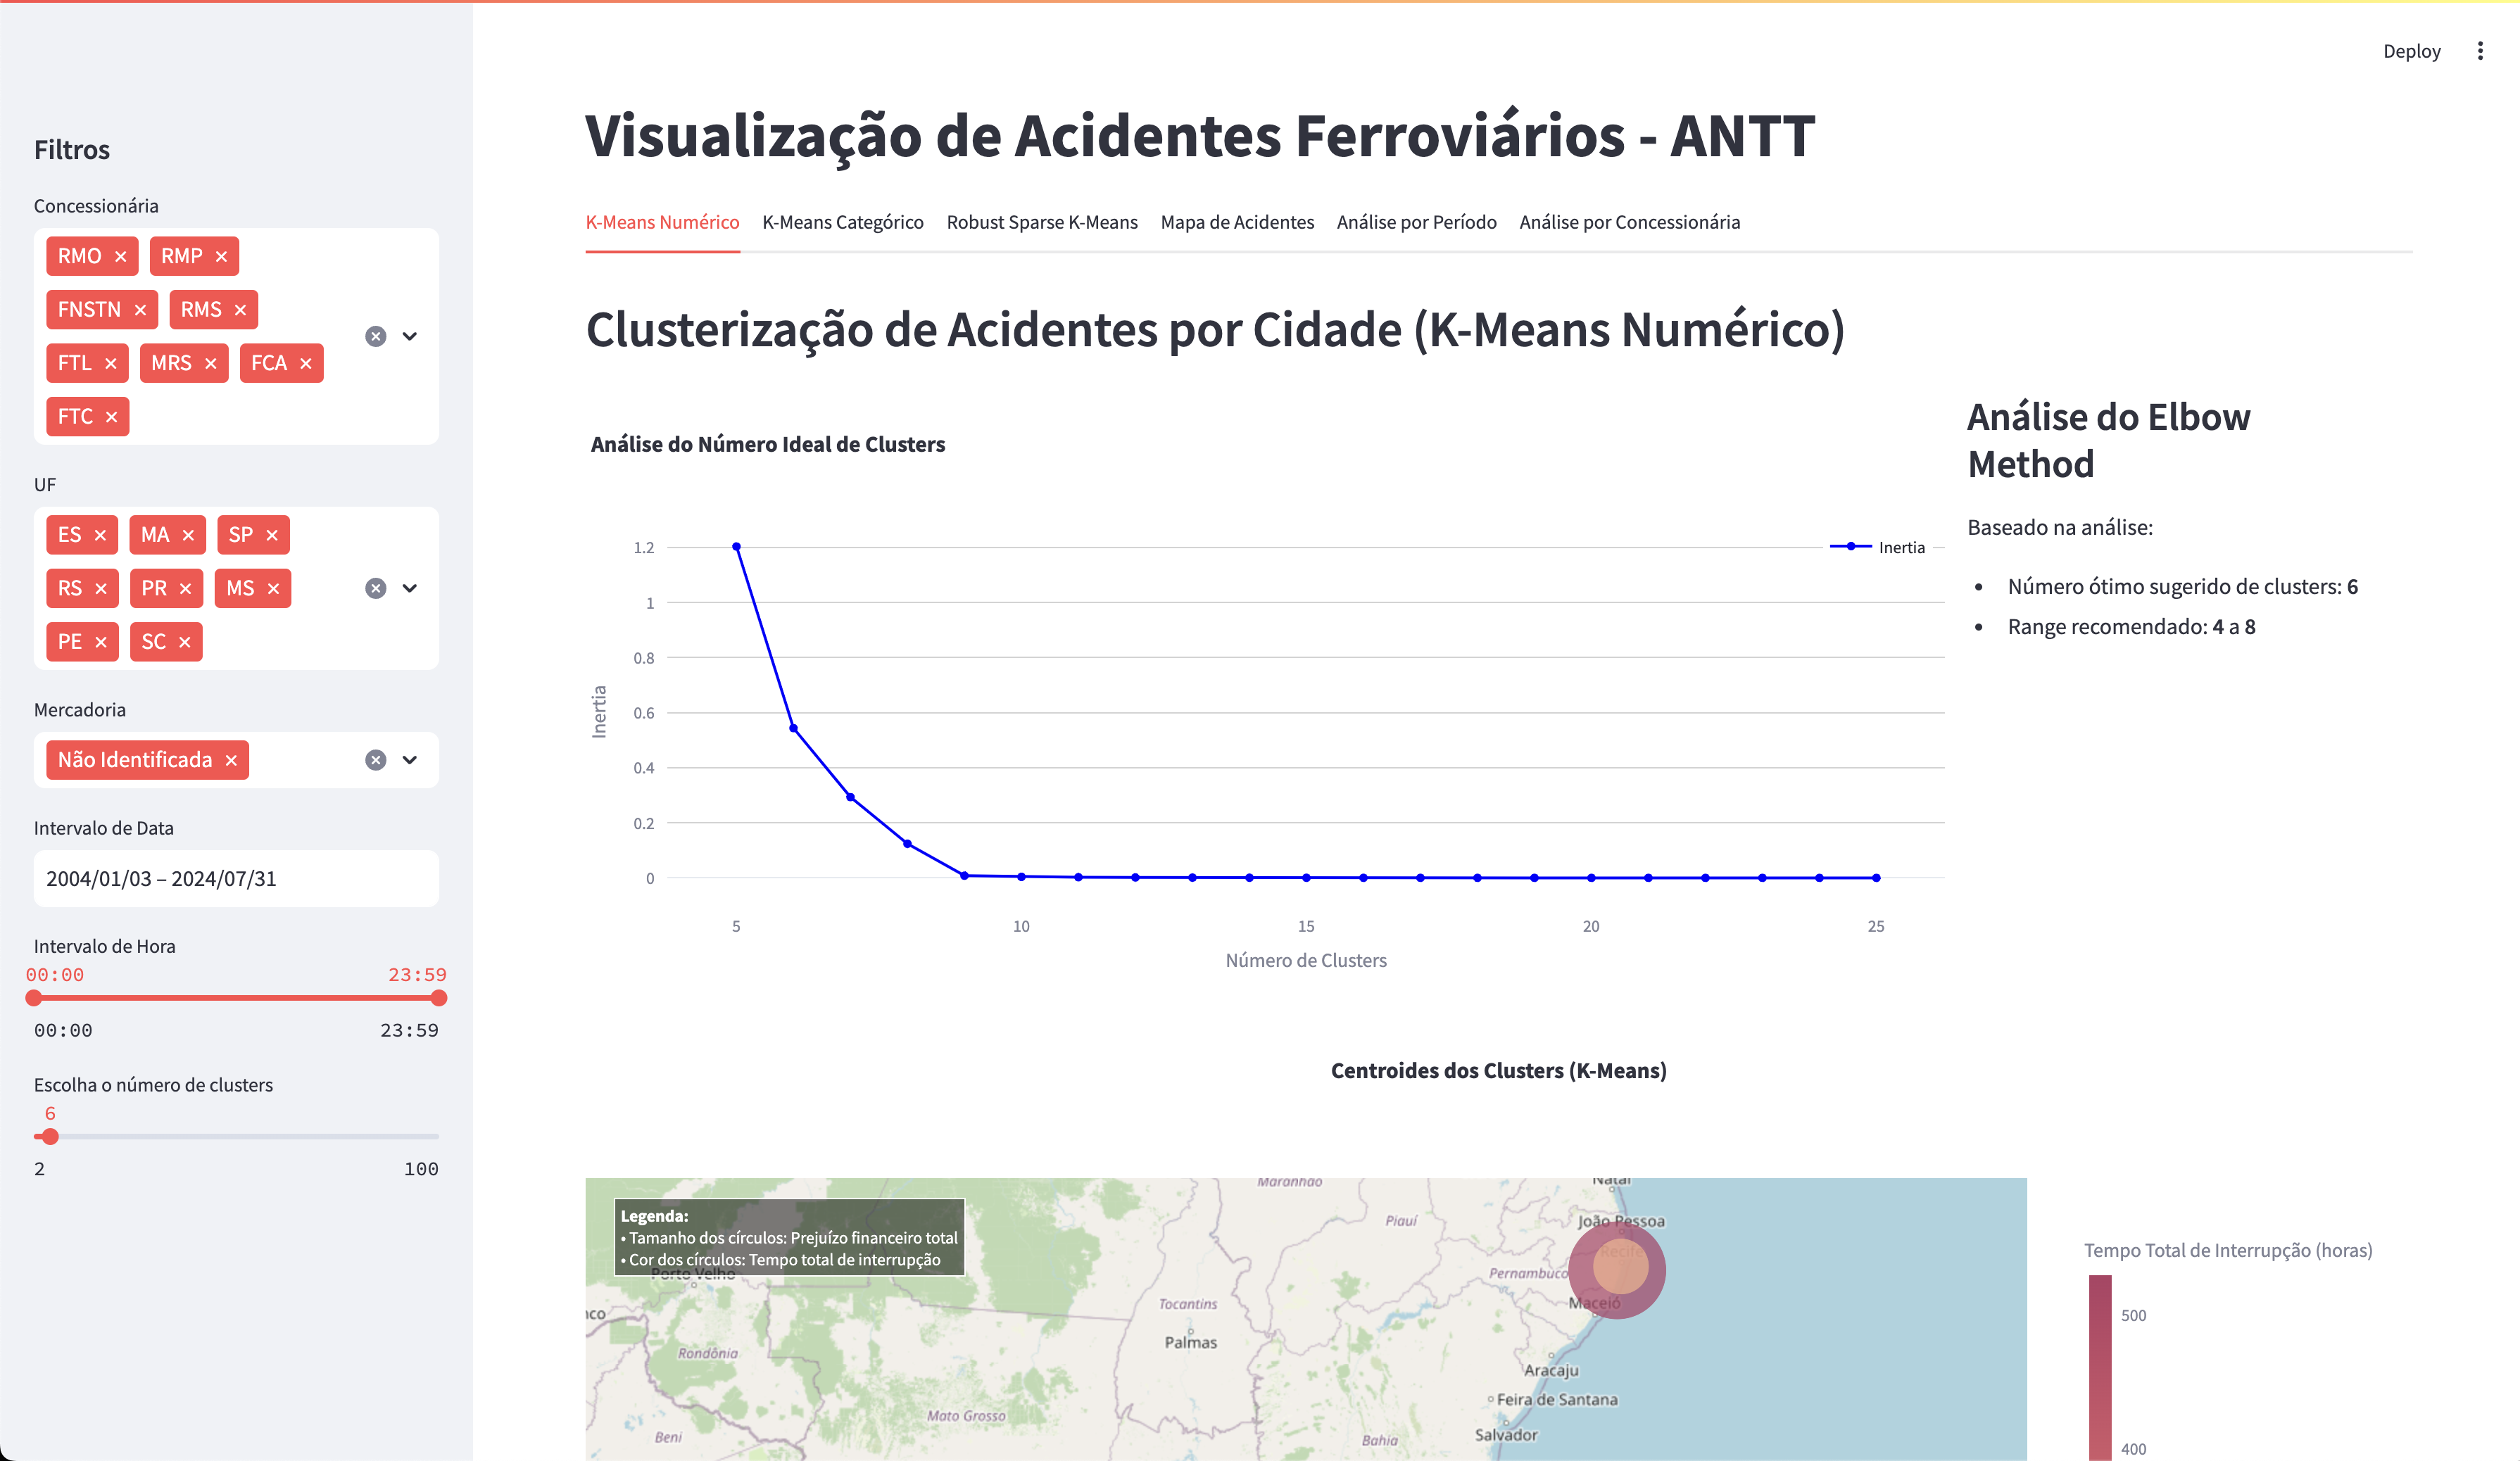
\includegraphics[width=0.9\linewidth]{sistema_interface.png}
    \caption{Interface principal do sistema de visualização, mostrando os controles interativos e o painel de visualização principal. Os filtros laterais permitem a seleção dinâmica de períodos, concessionárias e outras variáveis de interesse.}
    \label{fig:sistema_interface}
\end{figure}

\subsection{Análise por Concessionária}

O sistema permite análise detalhada por concessionária ferroviária, revelando padrões específicos de cada operadora, como pode-se ver na figura \ref{fig:analise_concessionaria}:

\begin{figure}[!htb]
    \centering
    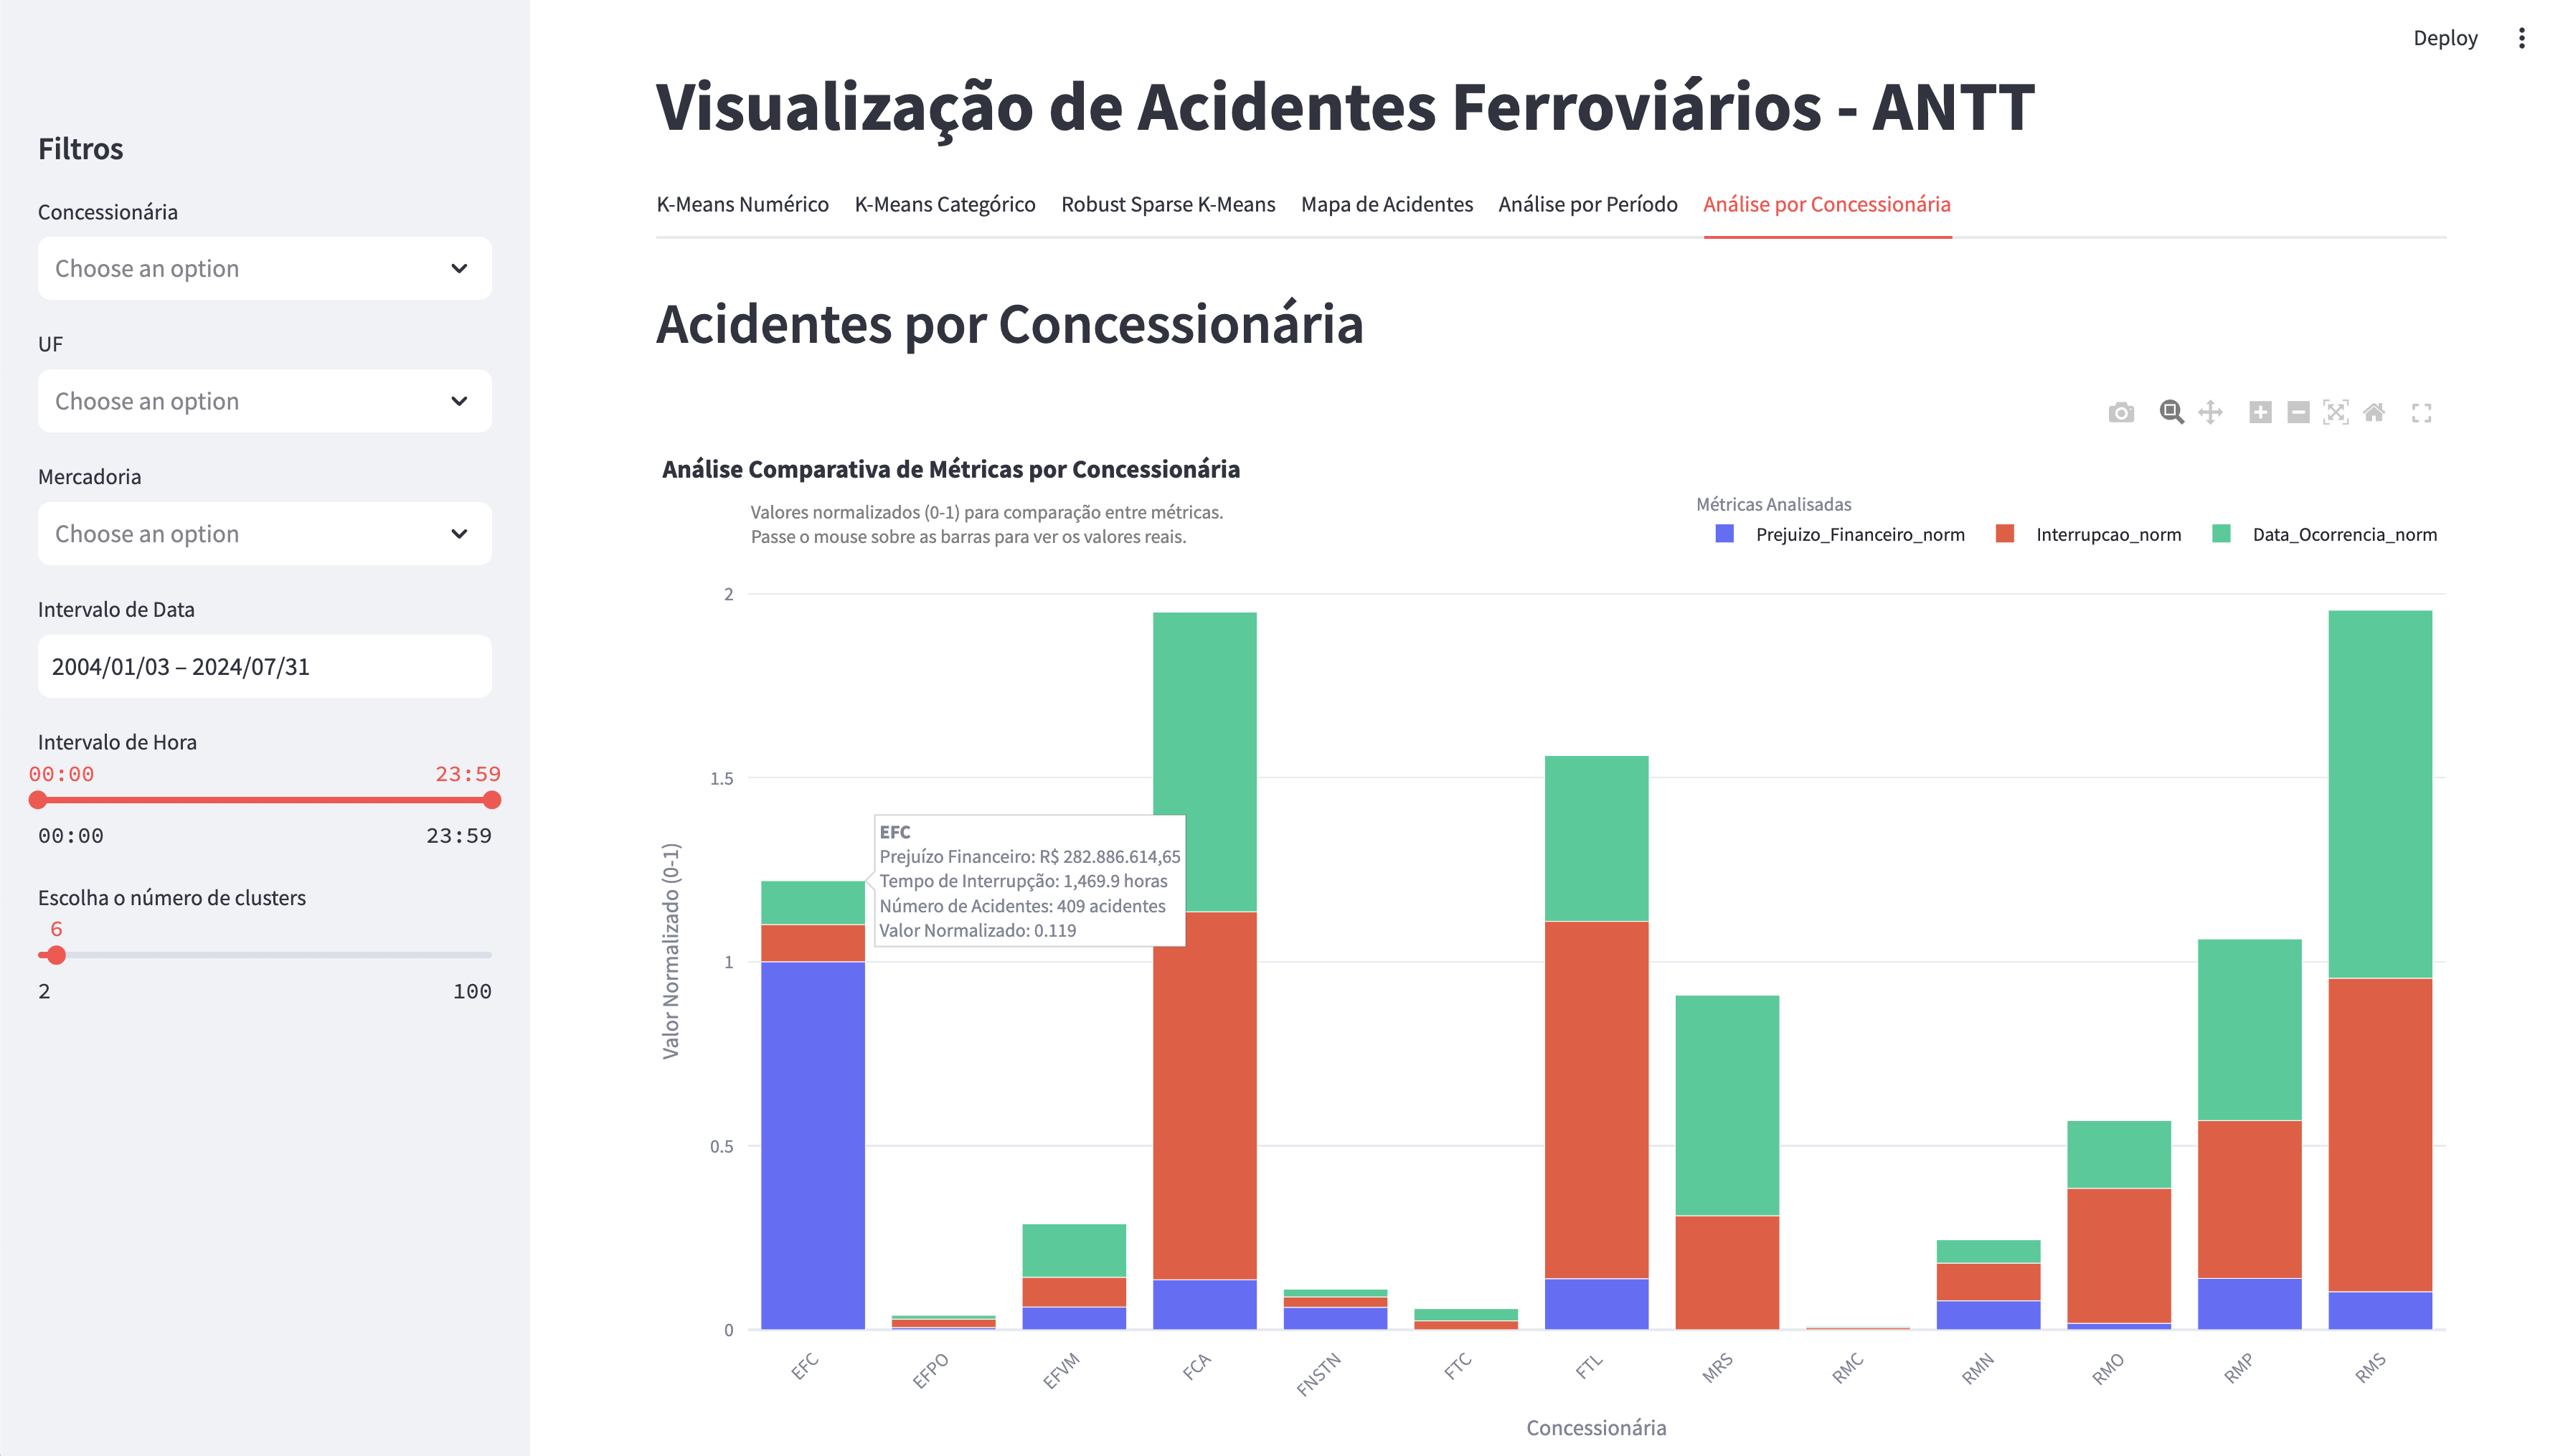
\includegraphics[width=0.8\linewidth]{analise_concessionaria.png}
    \caption{Visualização comparativa entre concessionárias, identificando métricas normalizadas de prejuízo financeiro, tempo de interrupção e número de acidentes, nota-se os padrões distintos entre operadoras.}
    \label{fig:analise_concessionaria}
\end{figure}

\subsection{Análise Temporal}

A dimensão temporal dos acidentes é explorada através de uma visualização específica demonstrada na figura \ref{fig:analise_temporal}.

\begin{figure}[H]
    \centering
    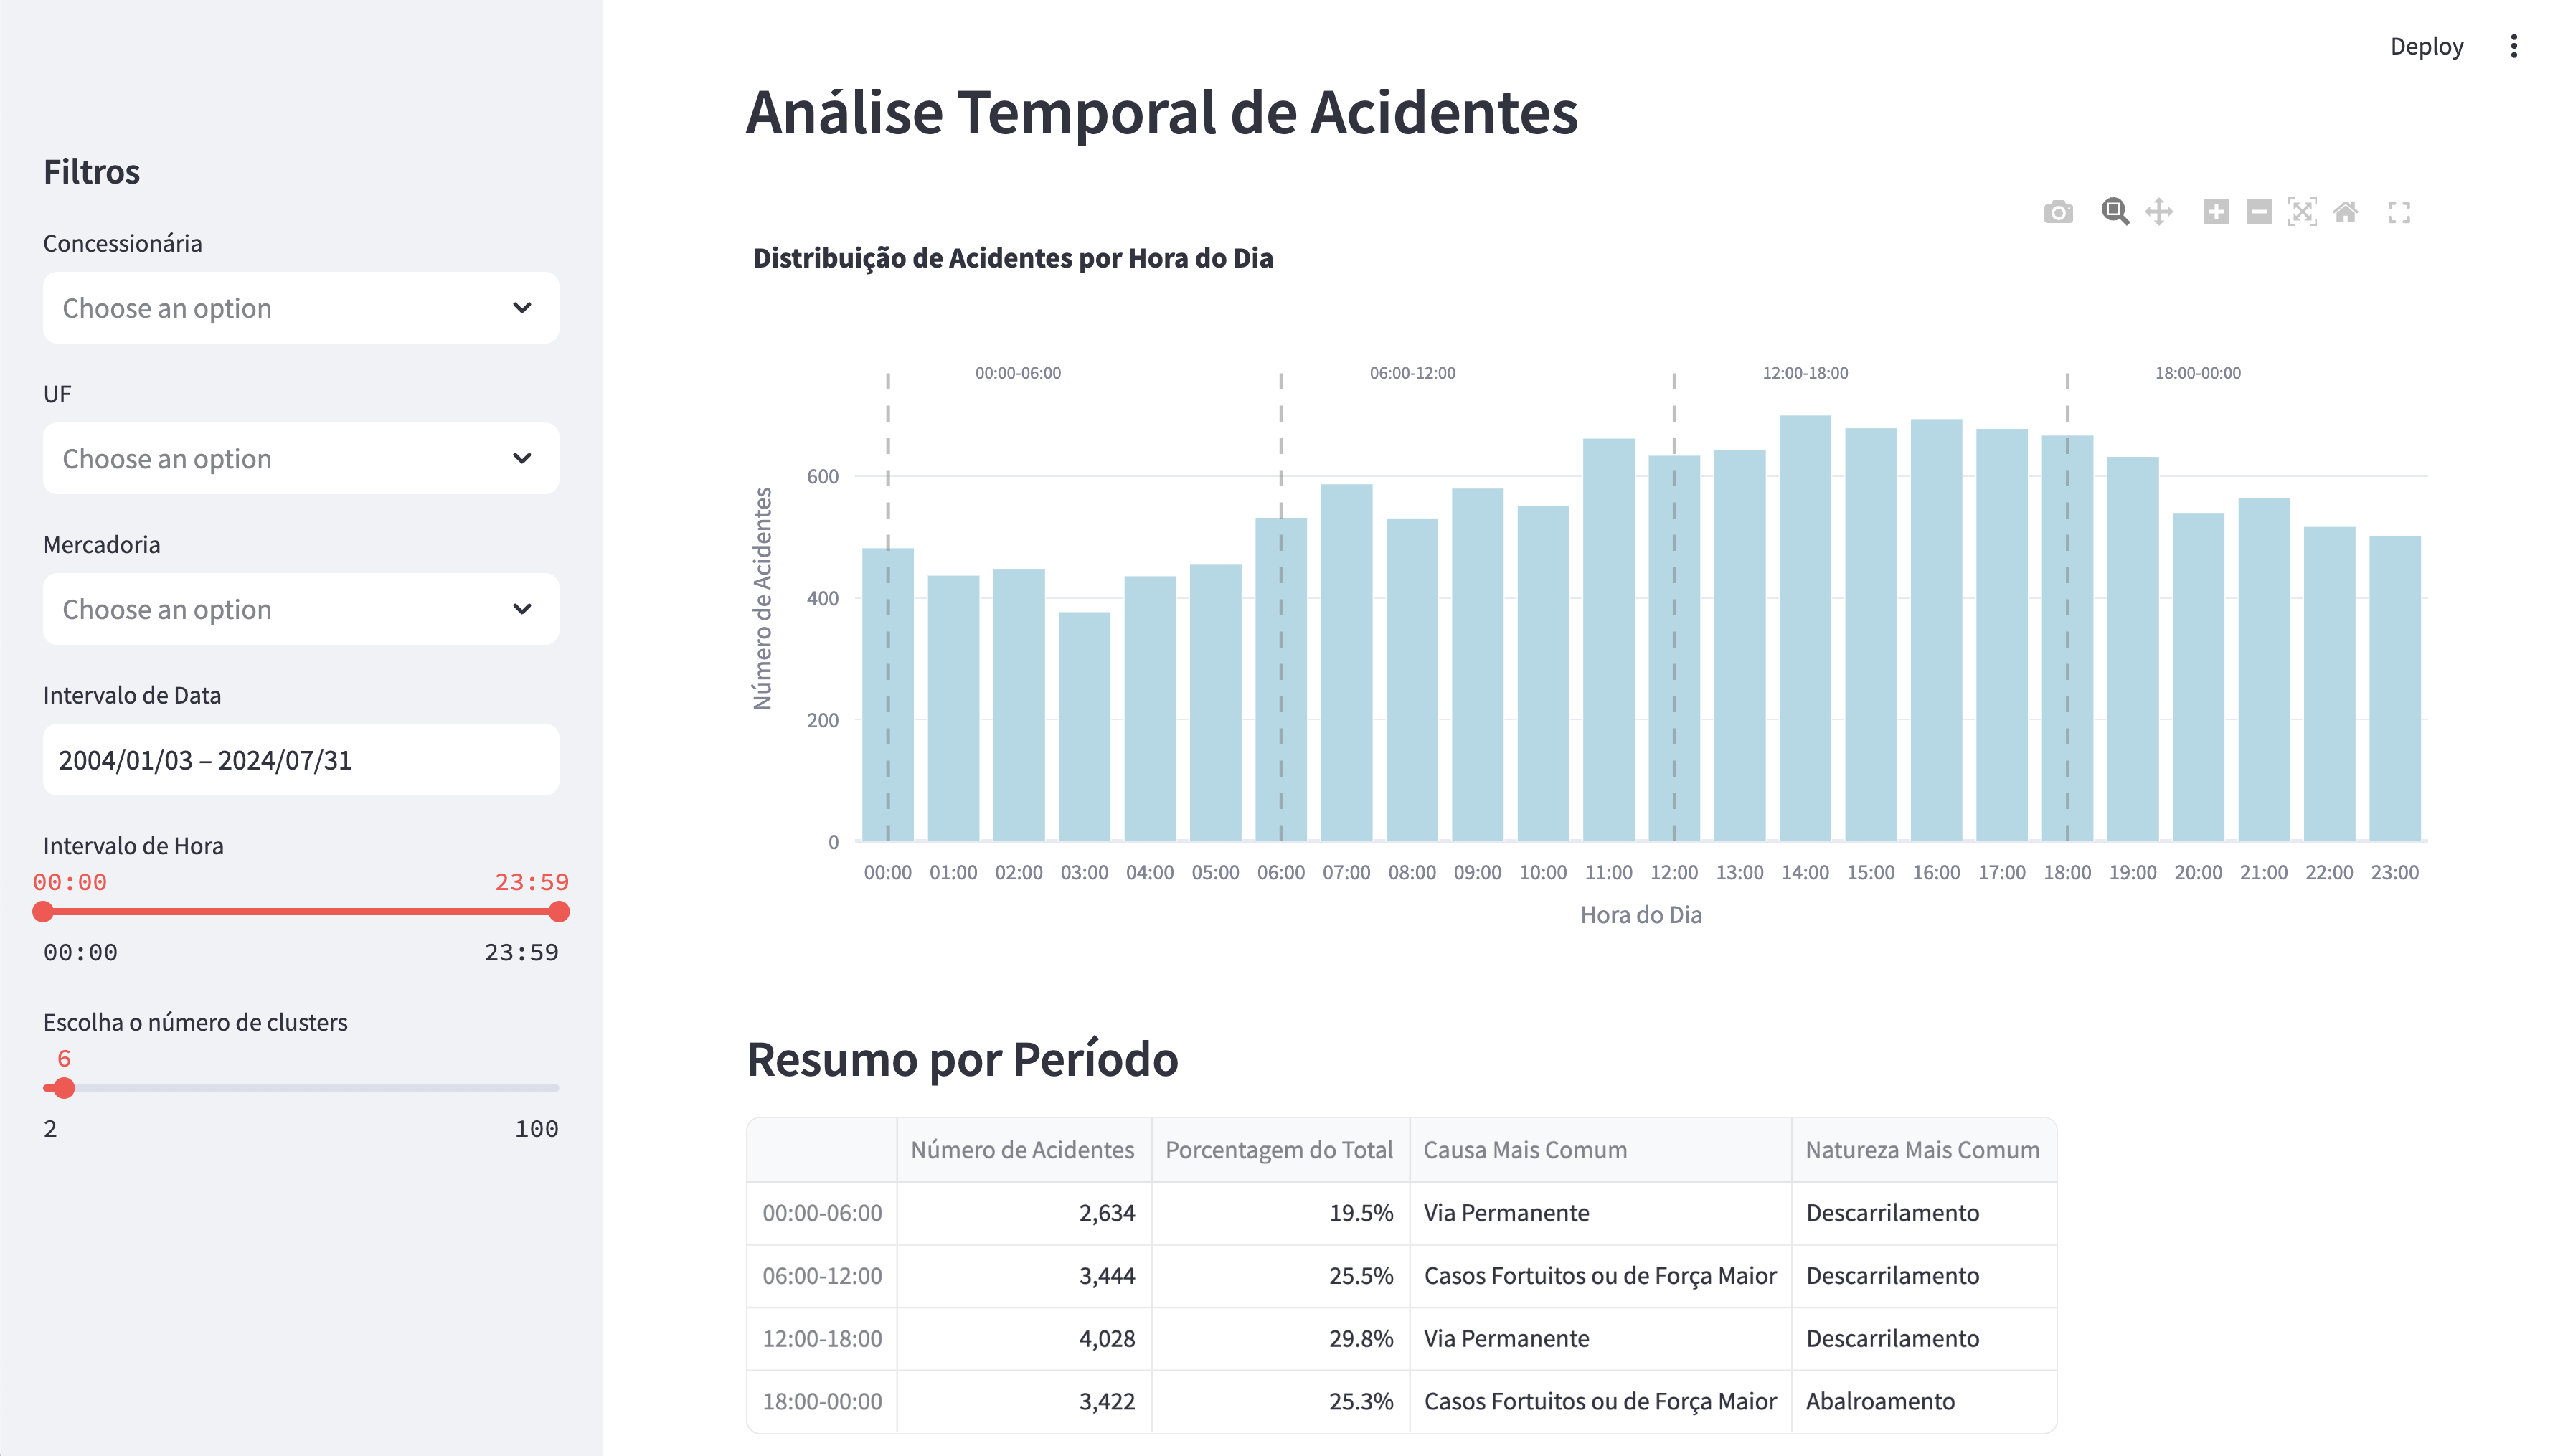
\includegraphics[width=0.8\linewidth]{analise_temporal.png}
    \caption{Distribuição temporal dos acidentes mostrando padrões horários e sazonais. Os gráficos de calor evidenciam concentrações de ocorrências em períodos específicos do dia e do ano.}
    \label{fig:analise_temporal}
\end{figure}

E também por meio de \textit{heatmaps} relacionando as características "Perímetro Urbano", "Causa Direta" e "Natureza", conforme demonstrado nas figuras \ref{fig:periodo_causa_direta}, \ref{fig:periodo_perimetro_urbano} e \ref{fig:periodo_natureza} respectivamente:

\begin{figure}[!htb]
    \centering
    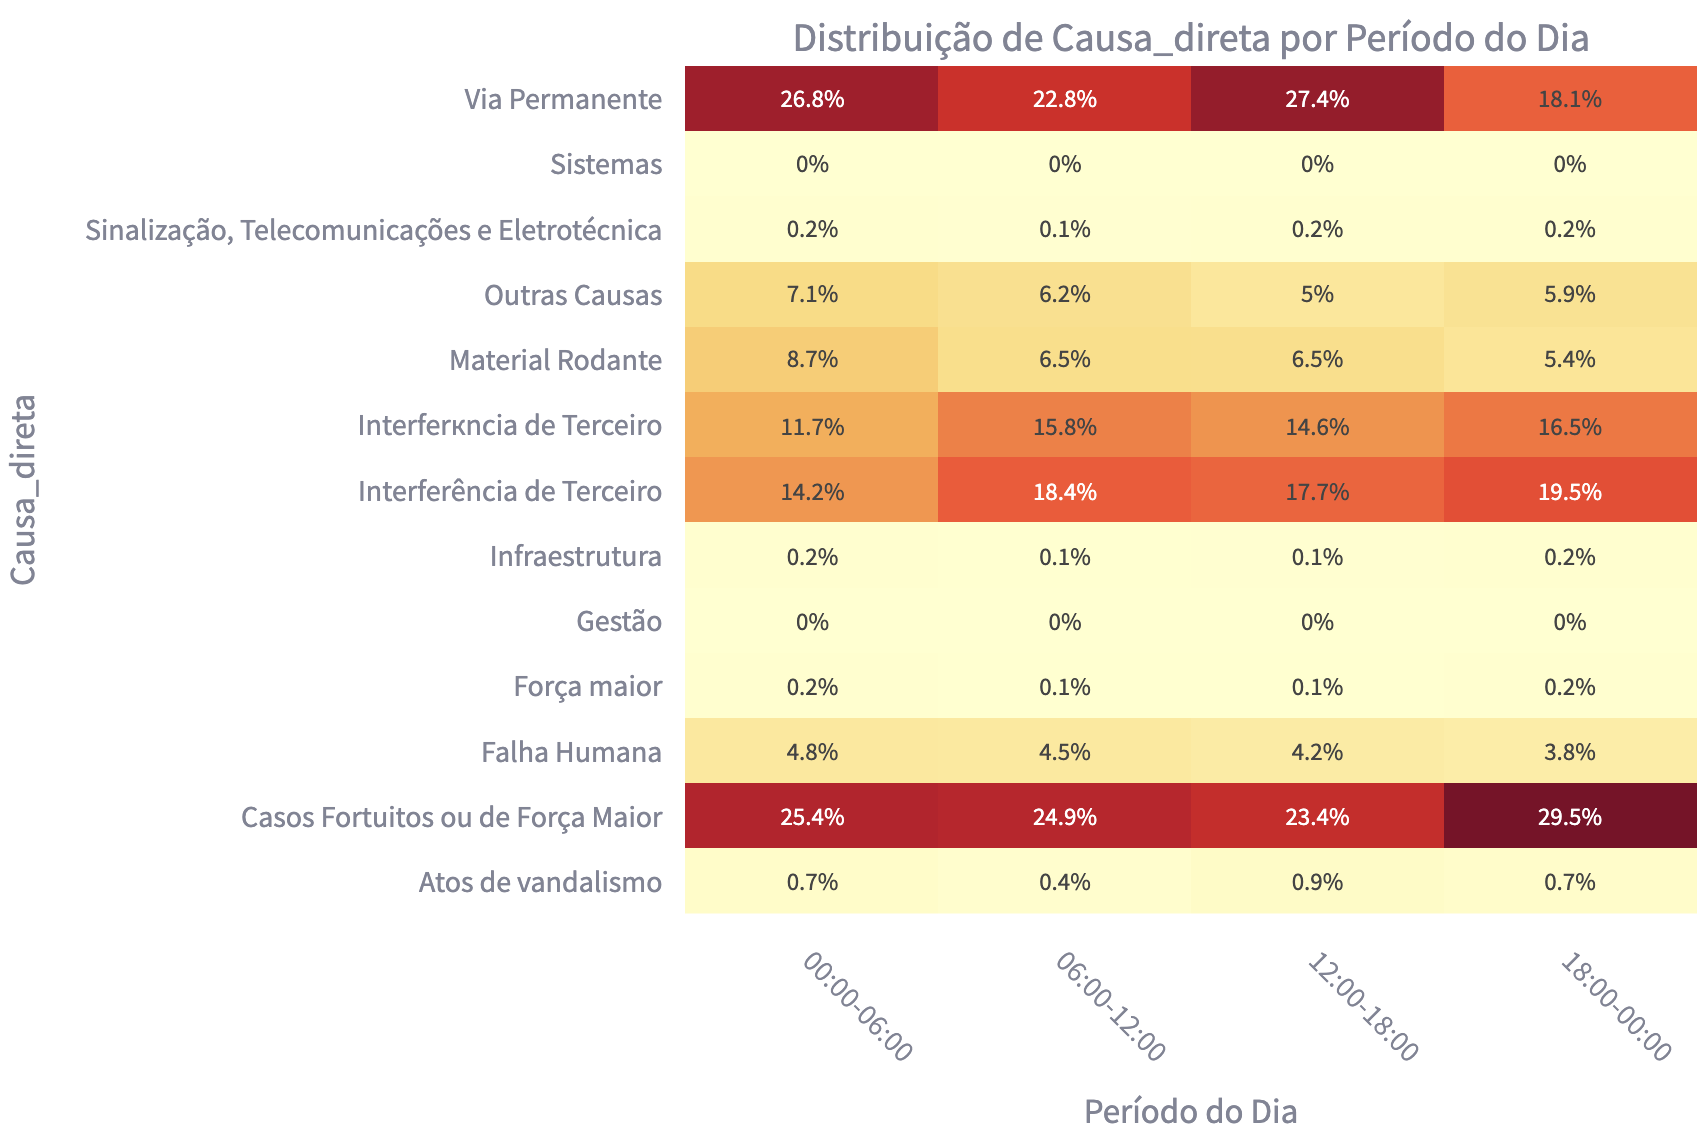
\includegraphics[width=0.9\linewidth]{periodo_causa_direta.png}
    \caption{Distribuição de Causa Direta por Período do Dia}
    \label{fig:periodo_causa_direta}
\end{figure}

\begin{figure}[!htb]
    \centering
    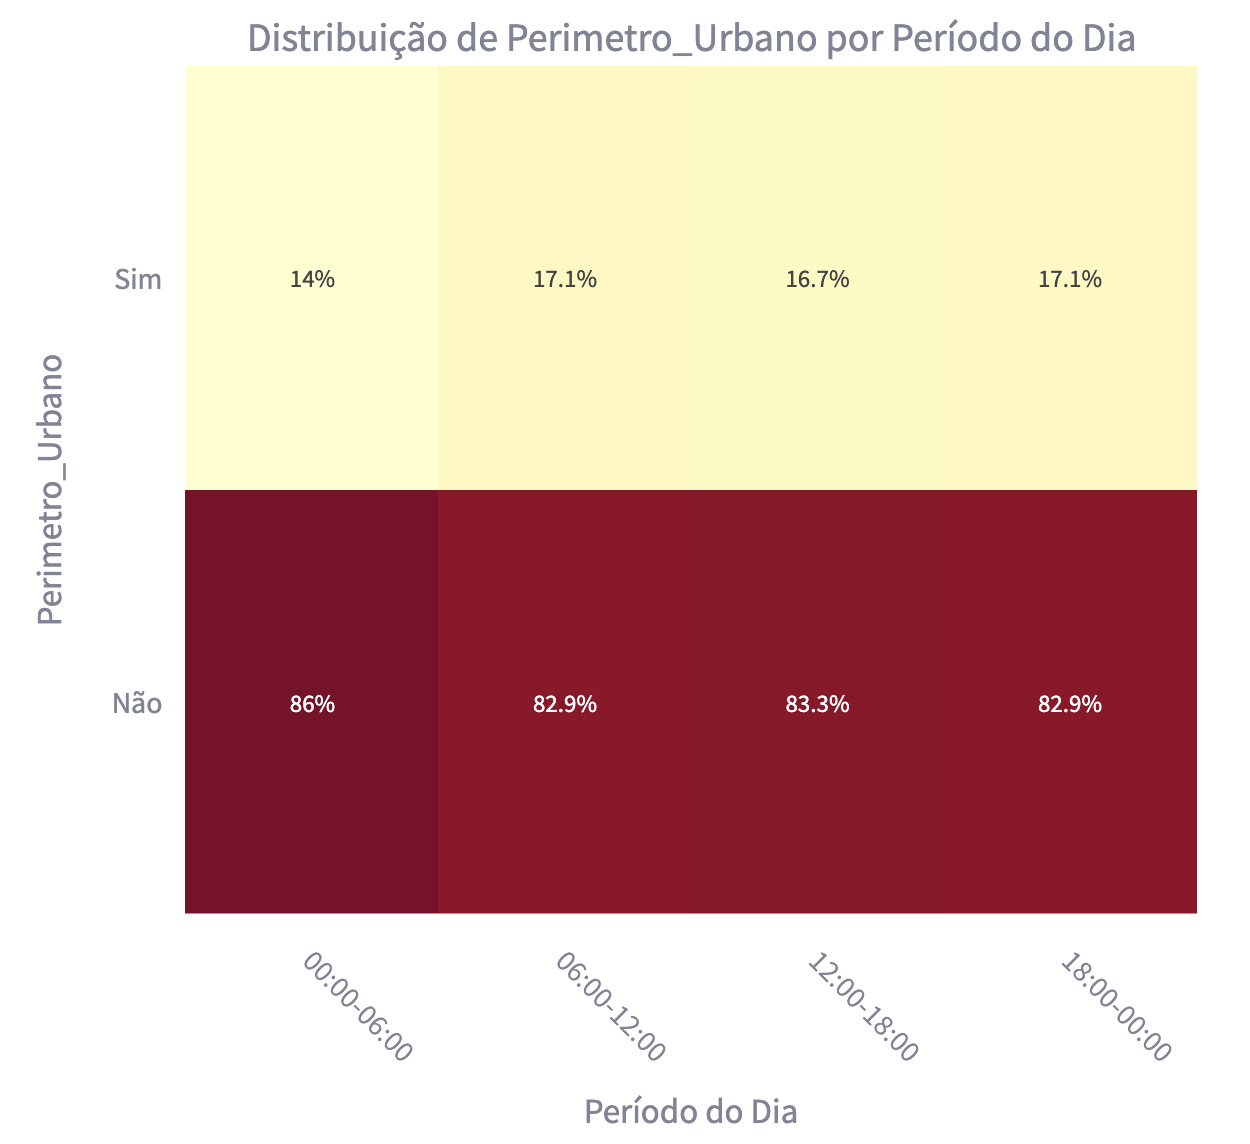
\includegraphics[width=0.95\linewidth]{periodo_perimetro_urbano.png}
    \caption{Distribuição de Perimetro Urbano por Período do Dia}
    \label{fig:periodo_perimetro_urbano}
\end{figure}

\begin{figure}[!htb]
    \centering
    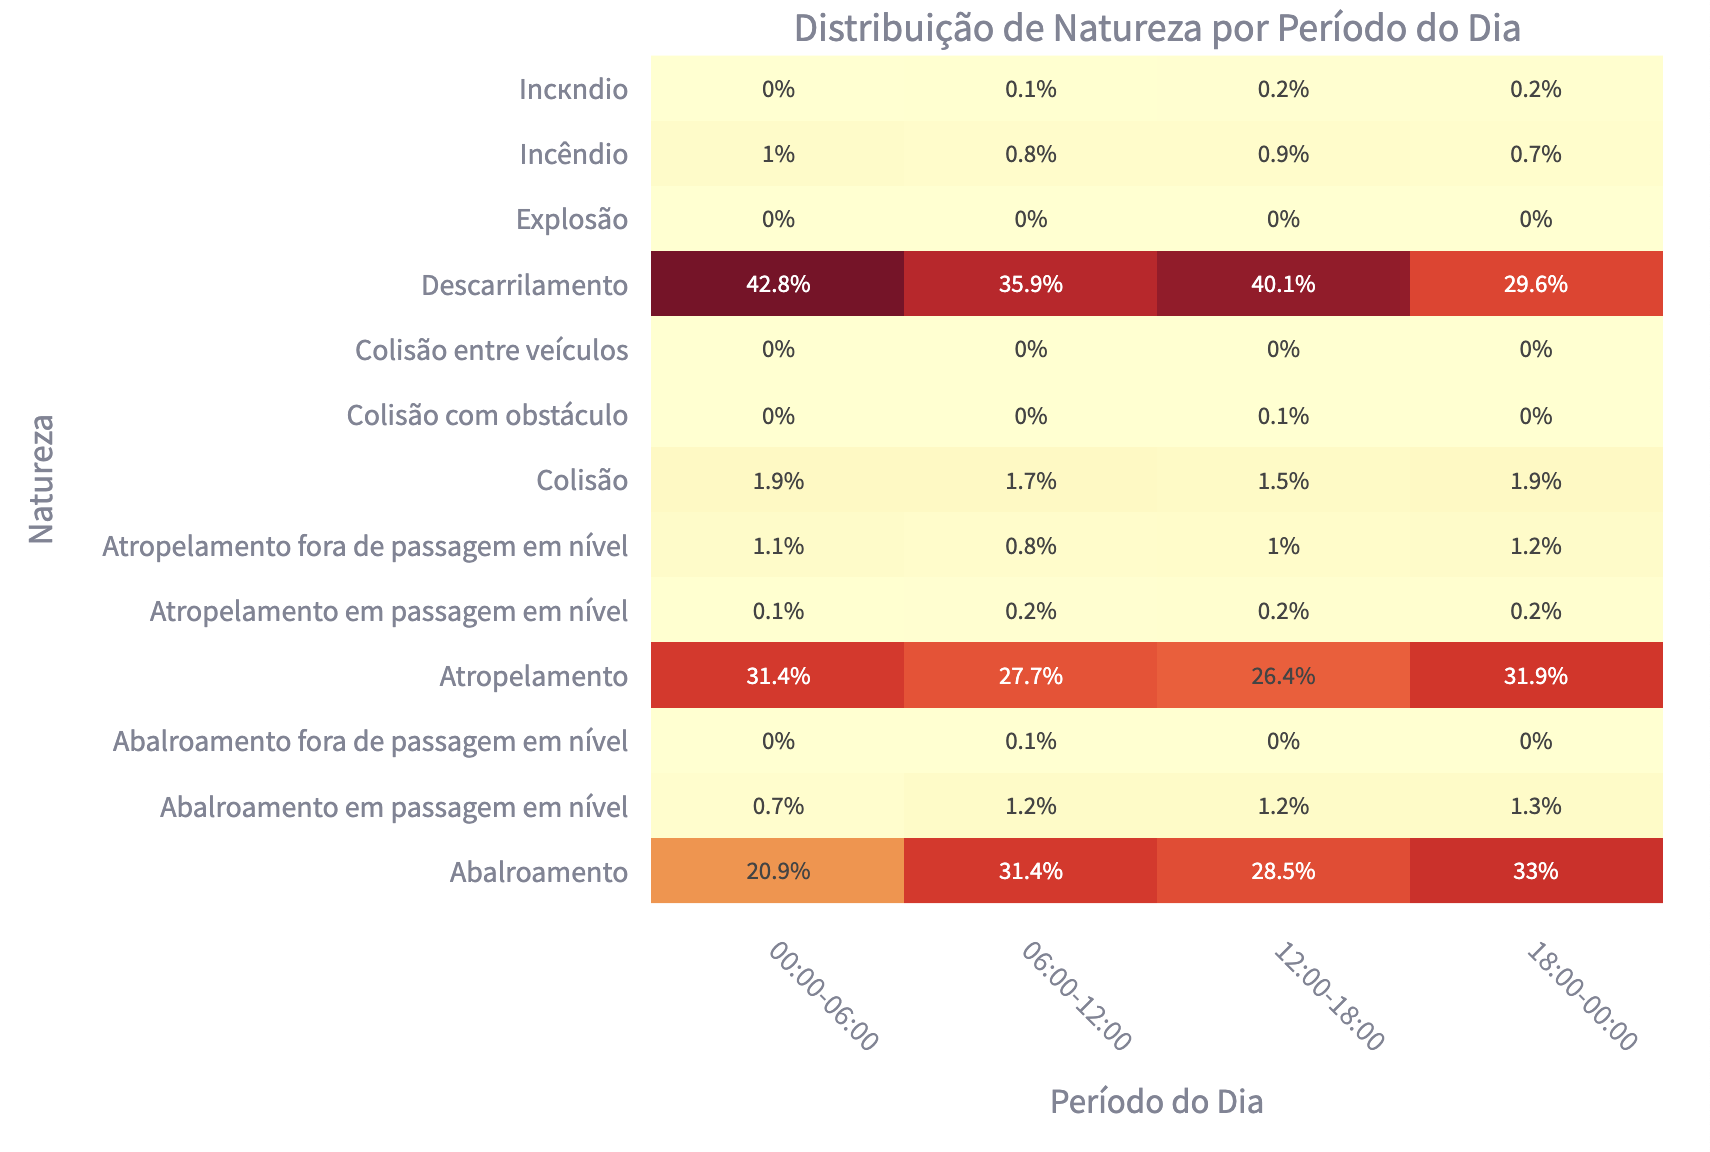
\includegraphics[width=0.95\linewidth]{periodo_natureza.png}
    \caption{Distribuição de Naturaza por Período do Dia}
    \label{fig:periodo_natureza}
\end{figure}

\section{Resultados}

\subsection{Análise Espacial}

\subsubsection{Distribuição Geográfica}
A análise da distribuição espacial dos acidentes ferroviários revela padrões significativos de concentração em determinadas regiões do Brasil. Através da visualização geoespacial interativa, foi possível identificar que a maior concentração de acidentes foi na região Sudeste e Sul do Brasil, como demonstra na figura \ref{fig:accident_map}.

\begin{figure}[h]
    \centering
    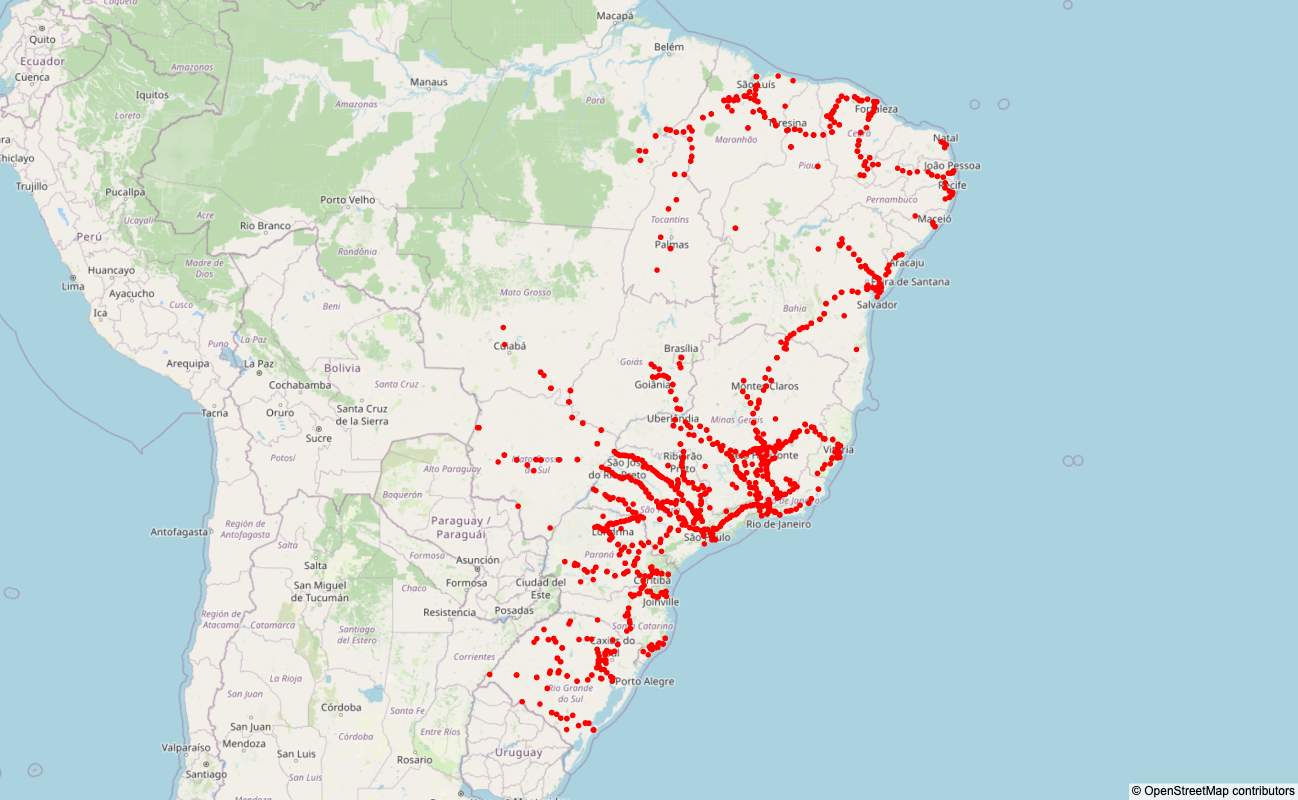
\includegraphics[width=0.99\linewidth]{accident_map.png}
    \caption{Mapa geográfico mostrando a distribuição geoespacial dos acidentes ferroviários no Brasil (2020-2024).}
    \label{fig:accident_map}
\end{figure}


\subsubsection{Padrões Regionais}
Os resultados demonstram uma concentração significativa de acidentes em corredores ferroviários específicos, particularmente em regiões com intensa atividade de transporte de carga. A análise comparativa entre as técnicas de \textit{clustering} revela padrões distintos de agrupamento, como mostrado nas Figuras \ref{fig:cluster_map} e \ref{fig:robust_sparse_kmeans}.

\begin{figure}[!htb]
    \centering
    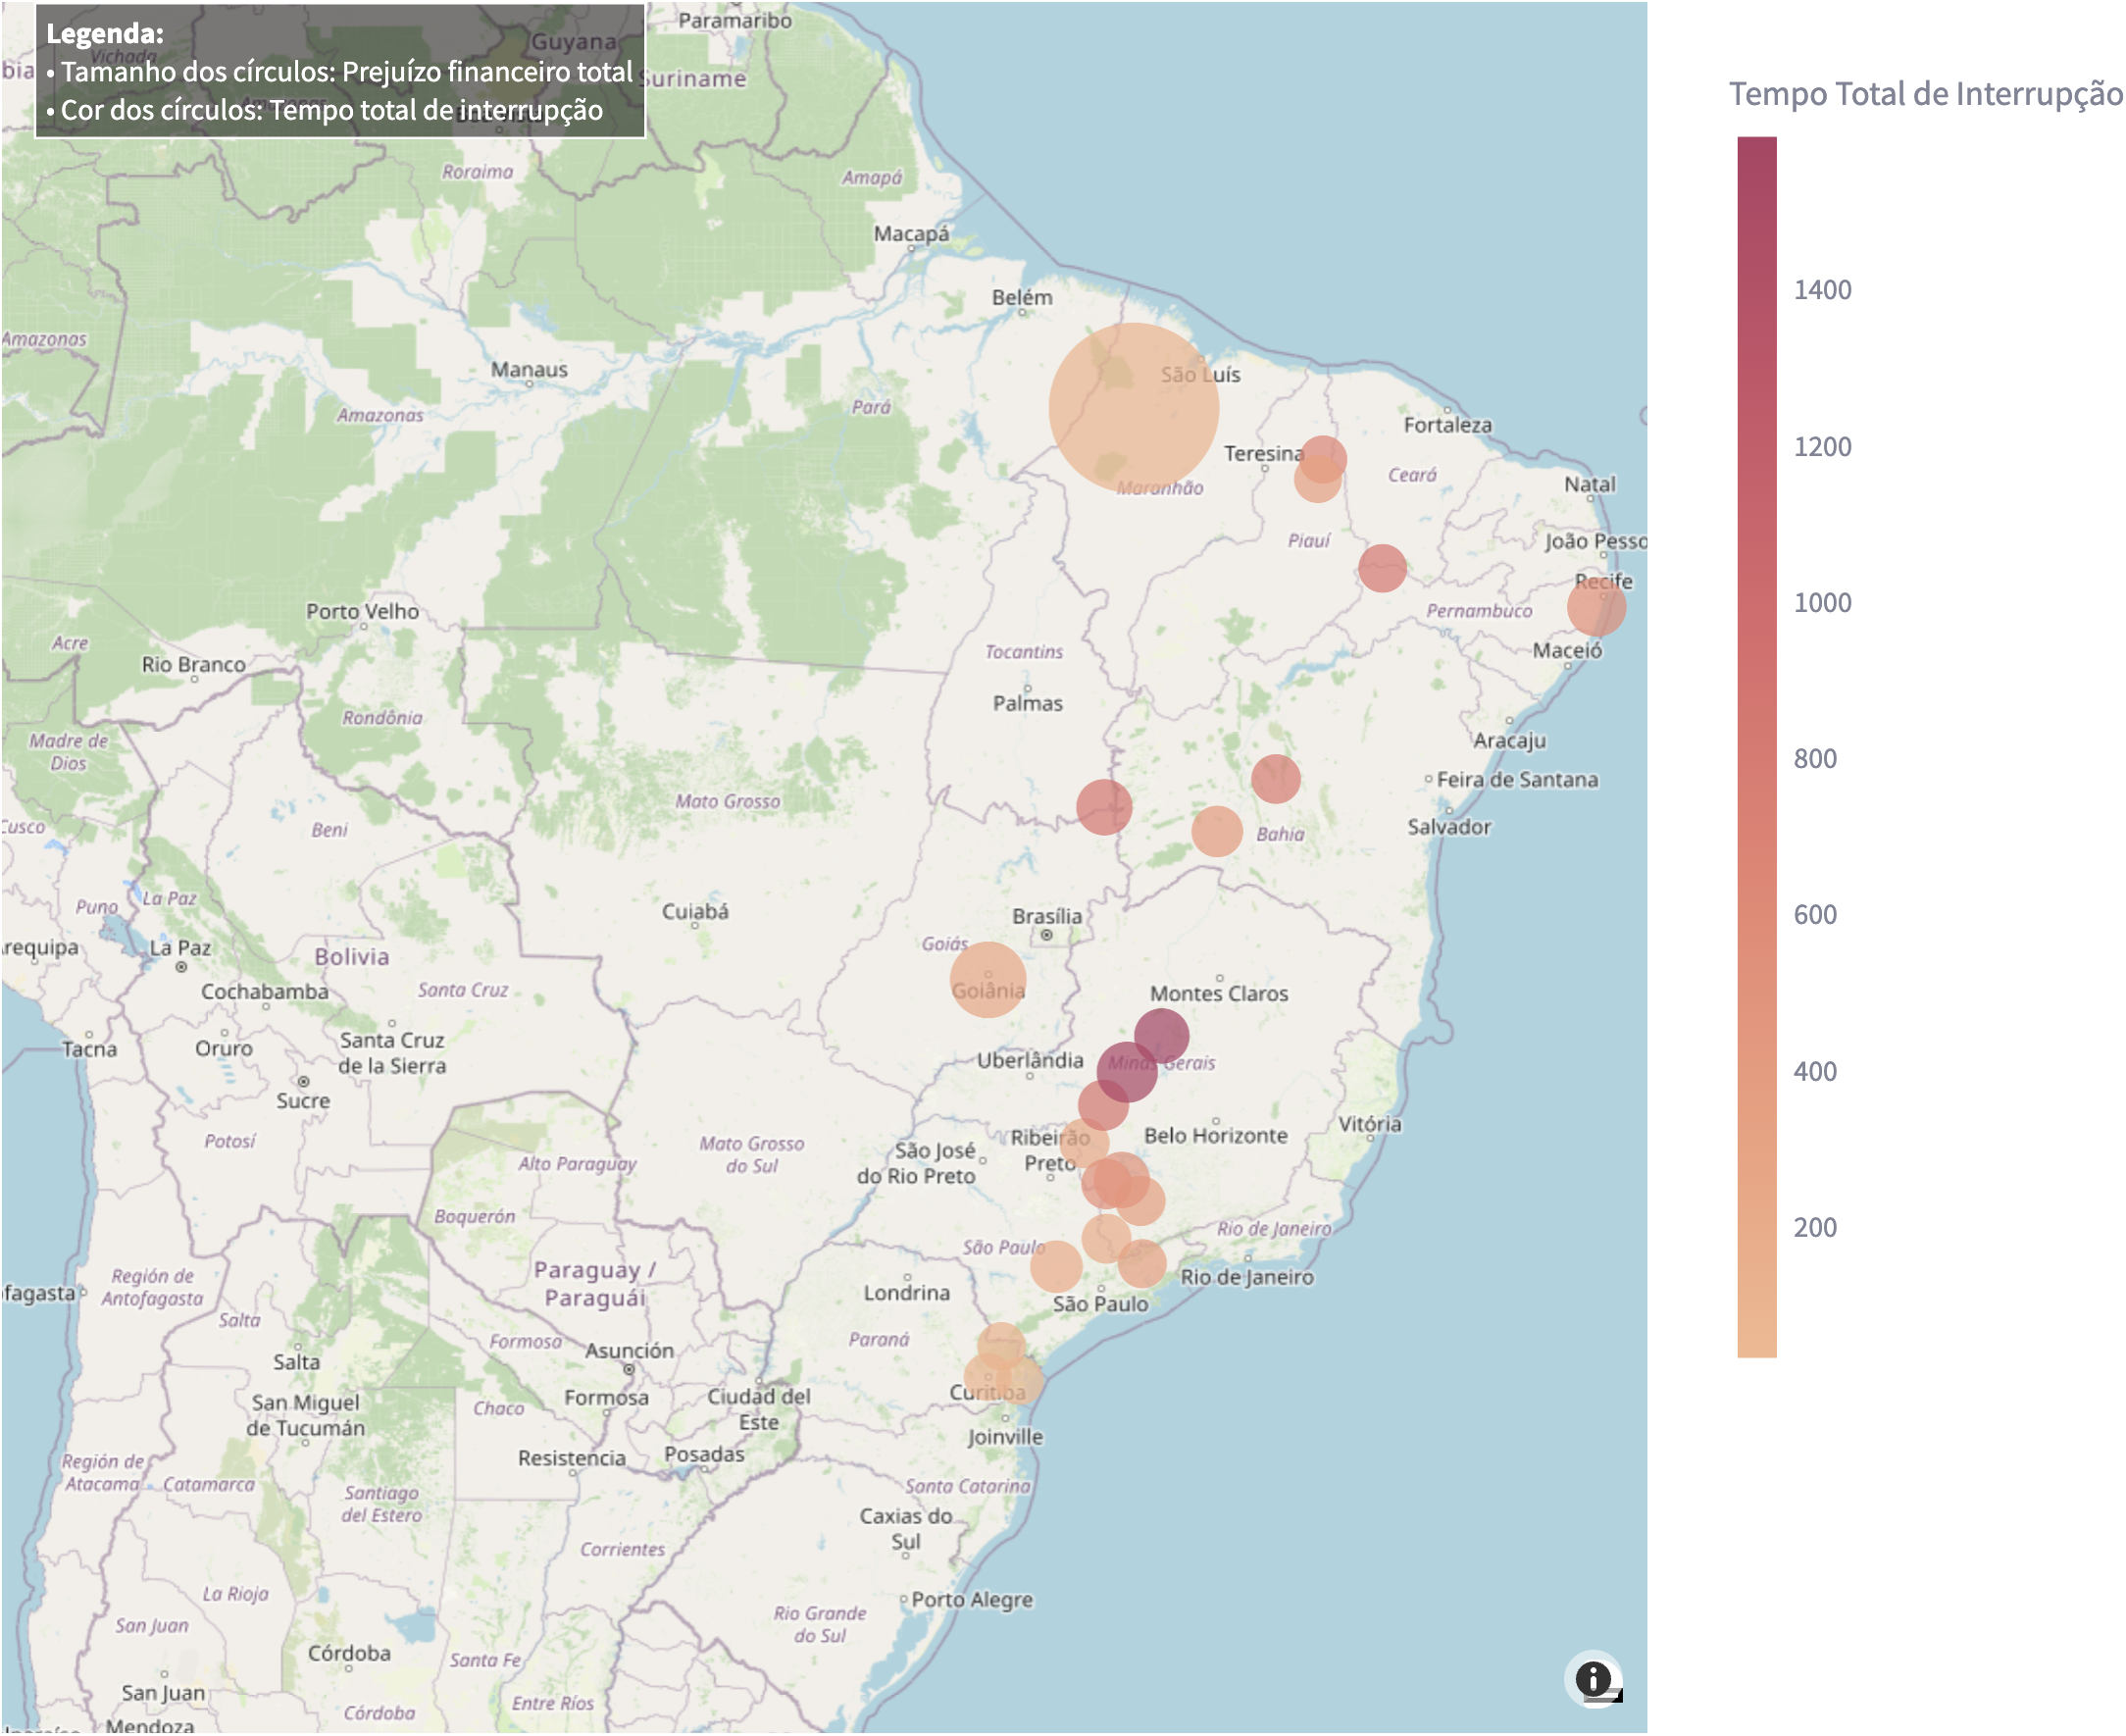
\includegraphics[width=0.99\linewidth]{kmeans_clustering.png}
    \caption{Visualização dos \textit{clusters} geográficos identificados pelo \textit{K-Means} tradicional. Cada ponto representa um centróide distinto, com o tamanho dos círculos proporcional ao prejuízo financeiro total e a intensidade da cor referente ao tempo de interrupção total.}
    \label{fig:cluster_map}
\end{figure}

\begin{figure}[!htb]
    \centering
    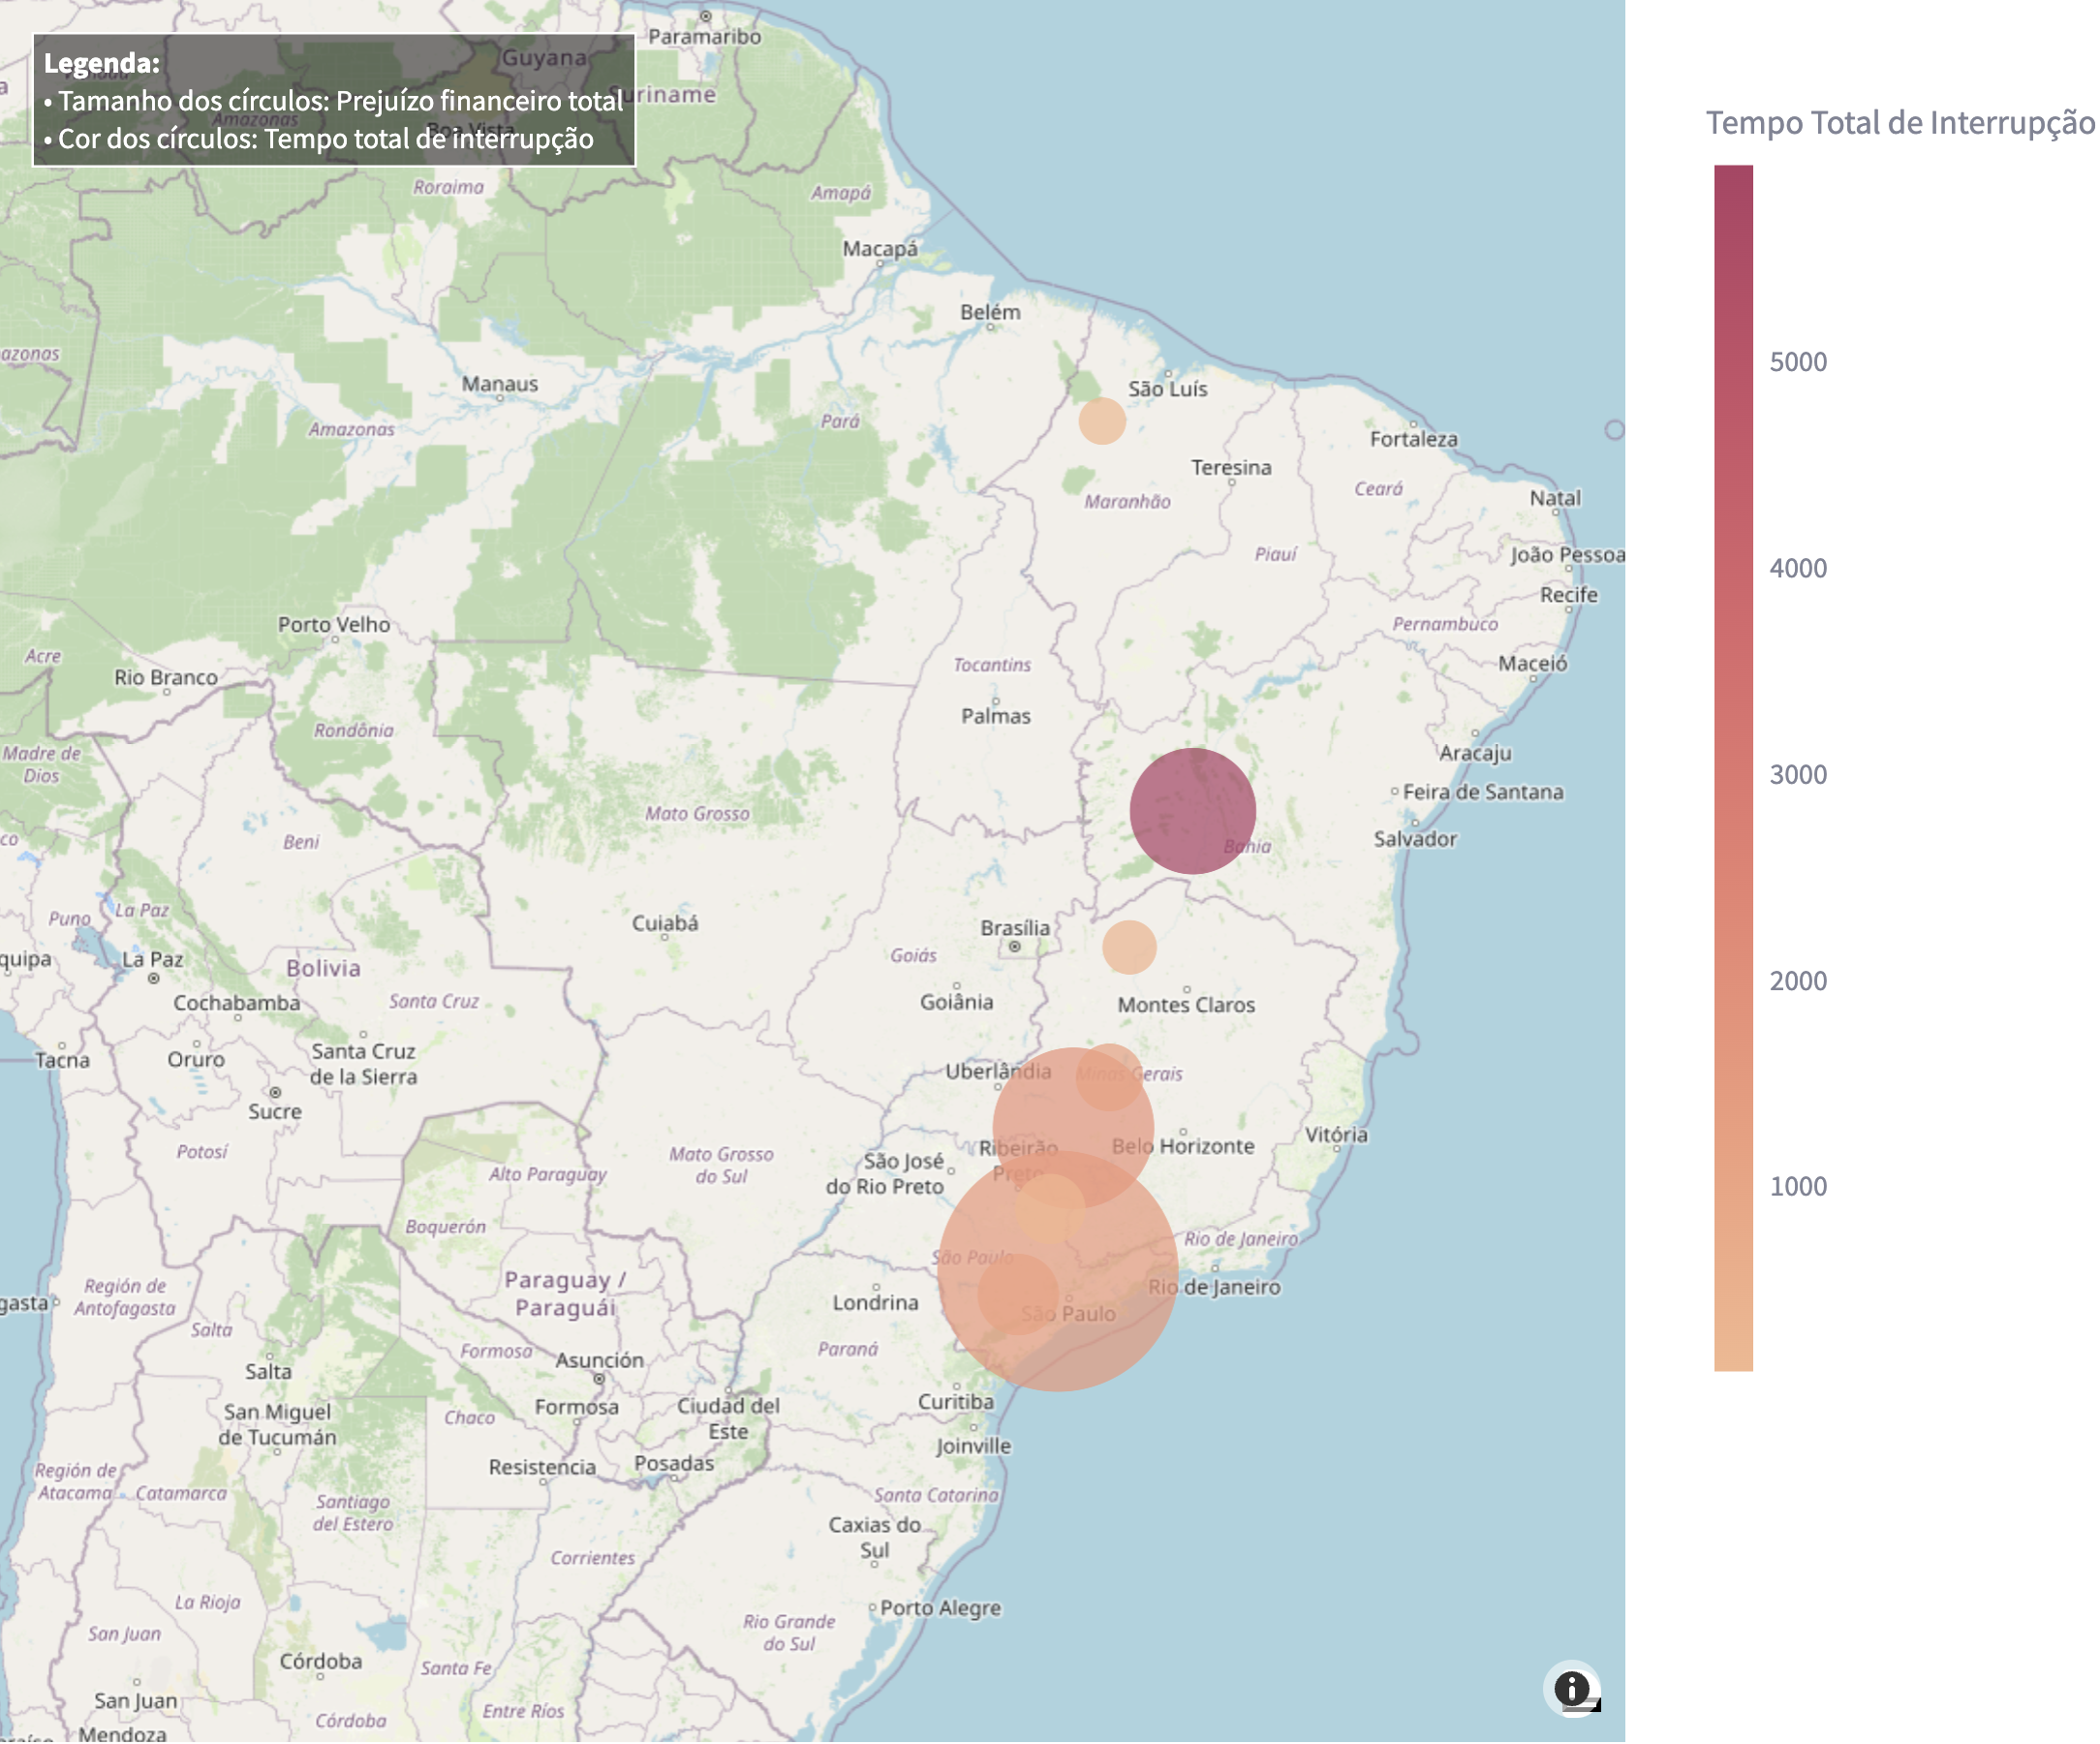
\includegraphics[width=0.99\linewidth]{robust_sparse_kmeans.png}
    \caption{Visualização dos \textit{clusters} geográficos identificados pelo \textit{Robust Sparse K-Means}. Cada ponto representa um centróide distinto, com o tamanho dos círculos proporcional ao prejuízo financeiro total e a intensidade da cor referente ao tempo de interrupção total. Note-se a redução significativa na influência de \textit{outliers} quando comparado à Figura \ref{fig:cluster_map}.}
    \label{fig:robust_sparse_kmeans}
\end{figure}

A análise dos padrões regionais revela quatro aspectos principais:

\begin{enumerate}
    \item \textbf{Concentração Geográfica:} Os \textit{clusters} identificados mostram uma forte concentração de acidentes ao longo dos principais corredores logísticos, especialmente nas regiões Sudeste e Sul do país.
    
    \item \textbf{Impacto Financeiro:} Os círculos de maior diâmetro, indicando maiores prejuízos financeiros, tendem a se concentrar em áreas de alta densidade operacional, sugerindo uma correlação entre volume de tráfego e magnitude dos impactos.
    
    \item \textbf{Tempo de Interrupção:} A intensidade da cor nos mapas revela que as regiões com maiores tempos de interrupção nem sempre coincidem com as áreas de maior prejuízo financeiro, indicando variações na eficiência dos processos de recuperação operacional.
    
    \item \textbf{Tratamento de \textit{Outliers}:} Comparando as Figuras \ref{fig:cluster_map} e \ref{fig:robust_sparse_kmeans}, é notável a diferença no tratamento de valores atípicos. O \textit{Robust Sparse K-Means} demonstra maior robustez ao reduzir significativamente a influência de \textit{outliers} na formação dos \textit{clusters}, resultando em uma representação mais coesa dos padrões regionais. Esta característica é particularmente evidente nas regiões periféricas, onde acidentes isolados ou eventos extremos têm menor impacto na definição dos centróides, proporcionando uma visão mais realista da distribuição típica dos acidentes.
\end{enumerate}

A robustez a \textit{outliers} demonstrada pelo \textit{Robust Sparse K-Means} é especialmente relevante no contexto de acidentes ferroviários, onde eventos extremos, embora importantes para análises específicas, podem distorcer a compreensão dos padrões gerais de ocorrências quando considerados com peso igual aos eventos mais frequentes.

\subsection{Análise de Desempenho dos Algoritmos}

A avaliação comparativa entre o \textit{K-Means} tradicional e o \textit{Robust Sparse K-Means} foi conduzida através de múltiplas perspectivas analíticas, incluindo métricas estabelecidas de qualidade de \textit{clustering} e análise aprofundada da importância das características através do \textit{framework} \textit{SHAP}. Esta abordagem multifacetada permitiu uma compreensão abrangente das forças e limitações de cada método no contexto específico da análise de acidentes ferroviários.

\subsubsection{Métricas de Avaliação}
A comparação quantitativa entre os algoritmos foi realizada utilizando três métricas complementares de avaliação, cada uma focando em diferentes aspectos da qualidade dos \textit{clusters}. O \textit{Silhouette Score}, introduzido por Rousseeuw \cite{rousseeuw1987silhouettes}, avalia a coesão interna dos \textit{clusters} e a separação entre \textit{clusters} diferentes. O \textit{Davies-Bouldin Index}, proposto por Davies e Bouldin \cite{davies1979cluster}, examina a similaridade entre \textit{clusters}, onde valores menores indicam melhor separação. O \textit{Calinski-Harabasz Score}, desenvolvido por Caliński e Harabasz \cite{calinski1974dendrite}, avalia a razão entre a dispersão intra e inter \textit{clusters}. A Tabela \ref{tab:clustering_metrics} apresenta os resultados comparativos dessas métricas.

\begin{table}[!htb]
    \centering
    \begin{tabular}{|l|c|c|}
        \hline
        \textbf{Métrica} & \textbf{K-Means} & \textbf{Robust Sparse K-Means} \\
        \hline
        Silhouette Score & 0.708 & 0.353 \\
        Davies-Bouldin Index & 0.408 & 1.205 \\
        Calinski-Harabasz Score & 10936.536 & 292.690 \\
        \hline
    \end{tabular}
    \caption{Comparação das métricas de avaliação entre \textit{K-Means} e \textit{Robust Sparse K-Means}}
    \label{tab:clustering_metrics}
\end{table}

Os resultados revelam um desempenho superior consistente do \textit{K-Means} tradicional em todas as métricas avaliadas:

\begin{itemize}
    \item \textbf{\textit{Silhouette Score}:} O \textit{K-Means} alcançou um \textit{score} de 0.708, significativamente superior ao 0.353 do \textit{Robust Sparse K-Means}. Segundo Rousseeuw \cite{rousseeuw1987silhouettes}, valores acima de 0.7 indicam uma estrutura forte de \textit{clustering}, sugerindo que o \textit{K-Means} conseguiu estabelecer \textit{clusters} bem definidos e coesos. O valor mais baixo do \textit{Robust Sparse K-Means} pode ser atribuído à sua tendência de criar \textit{clusters} mais especializados em determinadas características, potencialmente sacrificando a coesão geral em favor da robustez a \textit{outliers}.
    
    \item \textbf{\textit{Davies-Bouldin Index}:} O valor de 0.408 obtido pelo \textit{K-Means}, em contraste com 1.205 do \textit{Robust Sparse K-Means}, indica uma separação mais clara entre os \textit{clusters} no método tradicional. Davies e Bouldin \cite{davies1979cluster} estabelecem que valores menores deste índice sugerem \textit{clusters} mais bem separados e distintos. A diferença substancial entre os métodos sugere que o \textit{K-Means} foi mais eficaz em estabelecer fronteiras claras entre diferentes grupos de acidentes.
    
    \item \textbf{\textit{Calinski-Harabasz Score}:} A diferença mais pronunciada foi observada nesta métrica, com o \textit{K-Means} atingindo 10936.536 comparado a 292.690 do \textit{Robust Sparse K-Means}. Conforme estabelecido por Caliński e Harabasz \cite{calinski1974dendrite}, valores maiores indicam \textit{clusters} mais densos e bem separados. A magnitude desta diferença sugere que o \textit{K-Means} foi particularmente eficaz em maximizar a homogeneidade dentro dos clusters enquanto mantinha uma clara separação entre eles.
\end{itemize}

\subsubsection{Análise de Importância de Características com \textit{SHAP}}
Para interpretar o papel de cada variável na formação dos \textit{clusters}, empregou-se o método \textit{SHAP} (\textit{SHapley Additive exPlanations}) \cite{lundberg2017unified}, adaptado para o contexto de \textit{clustering}. Nesta abordagem, a contribuição de uma observação é definida como o negativo da distância mínima aos centróides dos \textit{clusters}. Formalmente, para um ponto \(x\), essa contribuição é dada por:
\[
\phi(x) = -\min_{k=1,\dots,K} \left\{ \sum_{j=1}^{p} w_{j}^{(k)} \left(x_j - \mu_{j}^{(k)}\right)^2 \right\},
\]
em que:
\begin{itemize}
    \item \(K\) representa o número de \textit{clusters};
    \item \(p\) é o número de características;
    \item \(\mu^{(k)}\) denota o centróide do \(k\)-ésimo \textit{cluster};
    \item \(w_{j}^{(k)}\) são os pesos atribuídos à característica \(j\), onde para o \textit{K-Means} tradicional \(w_{j}^{(k)}=1\) e, para o \textit{Robust Sparse K-Means}, os pesos são ajustados para enfatizar características de maior relevância.
\end{itemize}

Utilizando o \textit{KernelExplainer} do \textit{SHAP}, calcularam-se os valores médios absolutos de \(\phi(x)\) para cada característica, conforme demonstrado na Tabela \ref{tab:shap_comparison}. Esses valores quantificam a influência relativa de cada variável no processo de agrupamento.

\begin{table}[!htb]
    \centering
    \begin{tabular}{|l|c|c|}
        \hline
        \textbf{Característica} & \textbf{K-Means} & \textbf{Robust Sparse K-Means} \\
        \hline
        Interrupção & 0.572 & 0.941 \\
        Número de Acidentes & 0.608 & 0.744 \\
        Prejuízo Financeiro & 0.480 & 0.067 \\
        \hline
    \end{tabular}
    \caption{Valores médios absolutos de \textit{SHAP} para cada característica.}
    \label{tab:shap_comparison}
\end{table}

Observa-se que, para a variável \textbf{Interrupção}, o \textit{Robust Sparse K-Means} apresenta um valor médio absoluto de \textit{SHAP} de 0.941, superior ao 0.572 do \textit{K-Means} tradicional. Esse resultado indica que o algoritmo robusto atribui maior importância ao tempo de interrupção na formação dos \textit{clusters}, possivelmente por sua capacidade de destacar variáveis que melhor diferenciam os grupos.

De maneira similar, a variável \textbf{Número de Acidentes} possui valores de 0.608 e 0.744 para o \textit{K-Means} e o \textit{Robust Sparse K-Means}, respectivamente, sugerindo que o método robusto também enfatiza, de forma mais acentuada, a frequência de acidentes como fator determinante para a estruturação dos grupos.

Por outro lado, a variável \textbf{Prejuízo Financeiro} revela uma discrepância marcante: enquanto o \textit{K-Means} atribui um valor moderado (0.480) à sua contribuição, o \textit{Robust Sparse K-Means} registra um valor muito baixo (0.067). Essa diferença indica que o algoritmo robusto tende a minimizar a influência do prejuízo financeiro, possivelmente devido a uma menor variabilidade ou relevância dessa característica para a definição dos \textit{clusters}.

Em síntese, os resultados sugerem que o \textit{Robust Sparse K-Means} direciona sua atenção para variáveis que apresentam maior capacidade de
discriminação (como \textbf{Interrupção} e \textbf{Número de Acidentes}), ao mesmo tempo em que reprime aquelas de menor relevância (\textbf{Prejuízo Financeiro}). Tal comportamento é compatível com a finalidade dos métodos robustos e esparsos, que buscam realçar as características mais informativas e reduzir o impacto de variáveis menos contributivas.


\subsection{Análise Comparativa}

\subsubsection{Métricas de Qualidade dos \textit{Clusters}}
A comparação entre \textit{K-Means} tradicional e \textit{Robust Sparse K-Means} revelou diferenças significativas na qualidade dos agrupamentos, como pode-se ver nas figuras \ref{fig:elbow-plot-kmeans} e \ref{fig:elbow-plot-sparse-kmeans}.

\begin{figure}[!htb]
    \centering
    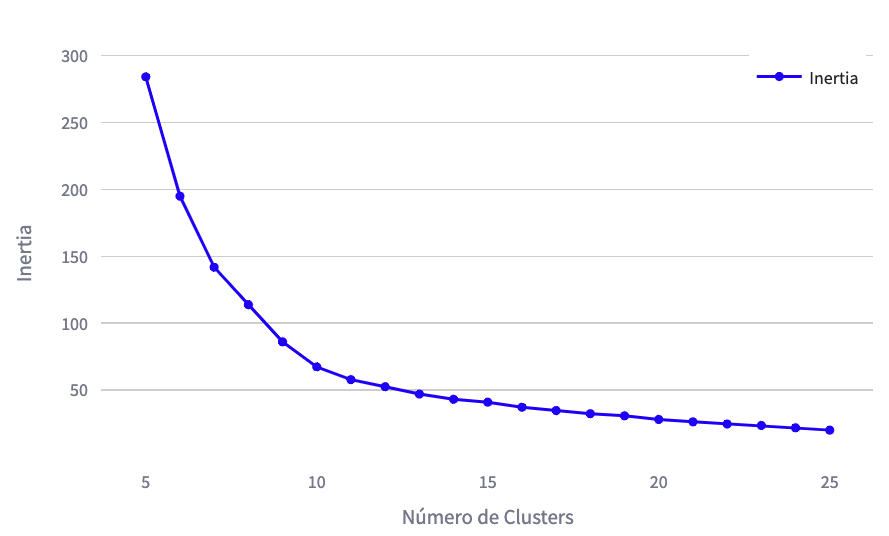
\includegraphics[width=0.9\linewidth]{elbow-plot-kmeans.png}
    \caption{Gráfico do método do cotovelo mostrando a variação da inércia em função do número de \textit{clusters} para o \textit{K-Means} tradicional}
    \label{fig:elbow-plot-kmeans}
\end{figure}

\begin{figure}[!htb]
    \centering
    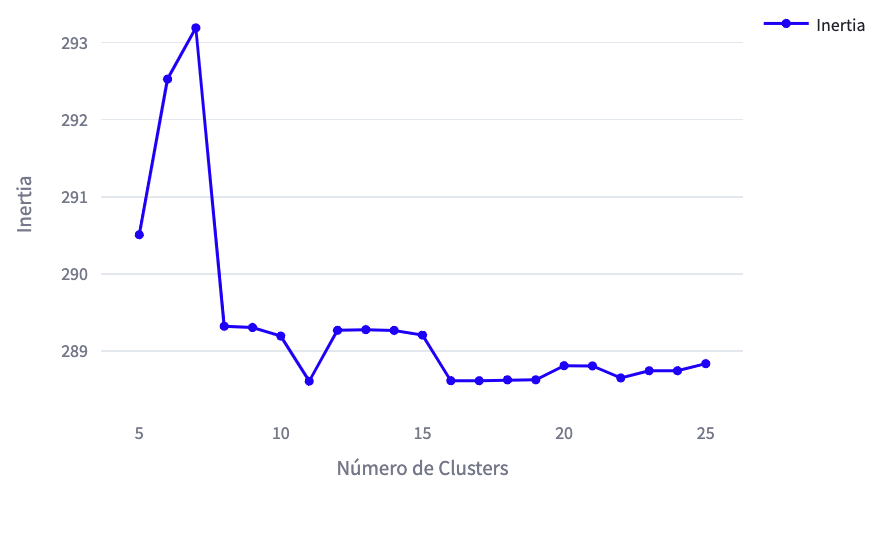
\includegraphics[width=0.8\linewidth]{elbow-plot-sparse.png}
    \caption{Gráfico do método do cotovelo mostrando a variação da inércia em função do número de \textit{clusters} para o \textit{Robust Sparse K-Means}
    \ref{fig:elbow-plot-kmeans}.}
    \label{fig:elbow-plot-sparse-kmeans}
\end{figure}


\subsection{Seleção de Características}

\subsubsection{Características Relevantes}
O \textit{Robust Sparse K-Means} identificou automaticamente as características mais relevantes para a formação dos \textit{clusters} através de sua capacidade de atribuir pesos às variáveis durante o processo de \textit{clustering}. A Tabela \ref{tab:feature_scores} apresenta os \textit{scores} de importância de cada característica, demonstrando que o prejuízo financeiro exerce influência dominante na formação dos agrupamentos, com um \textit{score} de 0.813, seguido pelo tempo de interrupção (0.442) e número de acidentes (0.380).

\begin{table}[!htb]
    \centering
    \begin{tabular}{|l|c|}
        \hline
        \textbf{Característica} & \textbf{\textit{Score} de Importância} \\
        \hline
        Prejuízo Financeiro & 0.813 \\
        Interrupção & 0.442 \\
        Número de Acidentes & 0.380 \\
        \hline
    \end{tabular}
    \caption[\normalfont{\textit{Scores} de importância das características}]{\textit{Scores} de importância das características identificadas pelo \textit{Robust Sparse K-Means}. Os valores são normalizados e refletem a contribuição relativa de cada variável para a formação dos \textit{clusters}.}
    \label{tab:feature_scores}
\end{table}

\subsubsection{Impacto na Análise}
A seleção automática de características proporcionou uma redução significativa na dimensionalidade dos dados sem perda significativa de informação. A análise dos \textit{scores} de importância revela aspectos fundamentais sobre os padrões de acidentes ferroviários:

\begin{itemize}

\item O prejuízo financeiro emerge como a característica mais influente, com um \textit{score} de 0.813, indicando que este fator é preponderante na diferenciação entre clusters. Esta dominância sugere que o impacto econômico dos acidentes é um indicador mais robusto para a identificação de padrões do que a frequência dos eventos em si.

\item O tempo de interrupção apresenta um \textit{score} intermediário de 0.442, demonstrando sua relevância secundária na formação dos \textit{clusters}. Este resultado é particularmente interessante pois indica que, embora significativo, o tempo de paralisação operacional não está necessariamente correlacionado de forma linear com o prejuízo financeiro.

\item O número de acidentes, com \textit{score} de 0.380, apresenta a menor influência entre as características analisadas. Este resultado sugere que a quantidade absoluta de ocorrências pode ser menos importante para a compreensão dos padrões de acidentes do que a severidade de seus impactos econômicos e operacionais.

\end{itemize}

Esta hierarquização automática das características fornece \textit{insights} valiosos para a gestão da segurança ferroviária, sugerindo que estratégias de prevenção e mitigação devem priorizar a redução do impacto financeiro dos acidentes, além de simplesmente buscar a redução de sua frequência.

    
\section{Discussão}

\subsection{Robustez Estatística}
A análise comparativa entre \textit{K-means} tradicional e \textit{Robust Sparse K-means} revelou diferenças significativas na capacidade de lidar com \textit{outliers} e na estabilidade dos \textit{clusters} formados. Um caso particularmente ilustrativo foi identificado nos registros da concessionária EFC (Estrada de Ferro Carajás), onde valores atípicos de prejuízos financeiros influenciaram significativamente a formação dos \textit{clusters} no \textit{K-means} tradicional.

O \textit{Robust Sparse K-means} demonstrou superior robustez estatística através de três aspectos principais:

1. \textbf{Tratamento de \textit{Outliers}:} Enquanto o \textit{K-means} tradicional mostrou-se sensível aos registros extremos da EFC, distorcendo a formação dos \textit{clusters} nas regiões próximas, o \textit{Robust Sparse K-means} manteve uma distribuição mais equilibrada dos centróides, preservando a representatividade dos padrões regionais típicos.

2. \textbf{Estabilidade dos \textit{Clusters}:} A incorporação da regularização LASSO resultou em agrupamentos mais estáveis, menos suscetíveis a variações nos valores extremos. Esta característica é particularmente relevante para a análise de acidentes ferroviários, onde eventos extraordinários não devem obscurecer padrões operacionais regulares.

3. \textbf{Consistência nas Métricas:} A variação da inércia em função do número de \textit{clusters} apresentou um comportamento mais suave no \textit{Robust Sparse K-means}, facilitando a identificação do número ótimo de \textit{clusters} através do método do cotovelo  \cite{b4}.

\subsection{Interpretabilidade}
A superioridade do \textit{Robust Sparse K-mean}s em termos de interpretabilidade manifesta-se em múltiplos níveis:

1. \textbf{Seleção Automática de características:} A atribuição de pesos às variáveis (\textit{scores} de 0.813 para prejuízo financeiro, 0.442 para interrupção e 0.380 para número de acidentes) fornece uma hierarquia clara de importância, facilitando a compreensão dos fatores mais relevantes na caracterização dos acidentes.

2. \textbf{Visualização Geoespacial:} A representação visual através do \textit{scatterplot} geolocalizado permite uma interpretação intuitiva dos padrões espaciais, com a vantagem adicional de que o \textit{Robust Sparse K-means} produz centróides mais representativos dos padrões típicos de cada região.

3. \textbf{Dimensionalidade Efetiva:} A redução automática da influência de variáveis menos relevantes simplifica a interpretação dos resultados, mantendo apenas as dimensões que efetivamente contribuem para a diferenciação entre clusters.

\subsection{Implicações Práticas}
A aplicação desta metodologia tem implicações significativas para a gestão da segurança ferroviária:

1. \textbf{Identificação de Prioridades:} A hierarquização das variáveis pelo \textit{Robust Sparse K-means} demonstrou uma identificação mais precisa e confiável dos padrões nos dados em comparação ao \textit{K-means} tradicional, especialmente ao lidar com valores atípicos e características complexas dos acidentes. Esta superioridade metodológica permitiu uma compreensão mais profunda das diferentes variáveis que caracterizam os acidentes ferroviários, oferecendo uma base mais sólida para o desenvolvimento de estratégias de segurança ferroviária.

2. \textbf{Gestão de Risco:} A capacidade de identificar padrões robustos, mesmo na presença de eventos extremos como os da EFC, permite uma avaliação mais precisa dos riscos típicos em diferentes regiões.

3. \textbf{Alocação de Recursos:} A visualização geoespacial dos clusters, combinada com os pesos das variáveis, fornece uma base objetiva para decisões sobre alocação de recursos de prevenção e resposta a acidentes.

\subsection{Comparação com Trabalhos Anteriores}
Nossa abordagem se diferencia e avança em relação a trabalhos anteriores em três aspectos principais:

1. \textbf{Integração de Técnicas:} A combinação de \textit{Robust Sparse K-means} com visualização geoespacial oferece uma perspectiva mais completa do que as abordagens tradicionais de análise de acidentes ferroviários.

2. \textbf{Tratamento de \textit{Outliers}:} A capacidade demonstrada de lidar com valores extremos, como os da EFC, representa um avanço significativo em relação a análises anteriores que frequentemente excluíam ou suavizavam estes casos.

3. \textbf{Interpretabilidade Aumentada:} A seleção automática de características e a visualização integrada proporcionam maior facilidade de interpretação do que os métodos anteriores.

\subsection{Análise dos Resultados de Importância das Características}

A análise da importância das características através do \textit{Robust Sparse K-means} revelou que o prejuízo financeiro exerce influência dominante na formação dos agrupamentos, com um \textit{score} de importância de 0,813. Este resultado estabelece um interessante paralelo com os achados de Pineda-Jaramillo et al. \cite{pineda2023short}, onde, utilizando uma abordagem diferente baseada em \textit{LightGBM} e \textit{SHAP}, também identificaram que variáveis relacionadas a impacto operacional e econômico têm peso significativo na caracterização de eventos ferroviários. Enquanto o estudo efetuado focou no impacto financeiro direto dos acidentes, Pineda-Jaramillo et al. \cite{pineda2023short}. demonstraram que o tempo de atraso na partida - uma variável com implicações financeiras indiretas - foi o preditor mais importante para atrasos futuros.

O alto \textit{score} de importância do impacto financeiro no presente trabalho (0,813) sugere que este fator é mais determinante na diferenciação entre \textit{clusters} do que a própria frequência dos eventos. Esta descoberta complementa a abordagem de Pineda-Jaramillo et al. \cite{pineda2023short}, que utilizaram gráficos de dependência \textit{SHAP} para visualizar como diferentes variáveis interagem na previsão de atrasos, demonstrando que impactos operacionais tendem a ter efeitos em cascata com implicações financeiras significativas.


\section{Conclusão}

A análise comparativa entre o \textit{K-means} tradicional e o \textit{Robust Sparse K-mean}s na investigação de acidentes ferroviários demonstrou significativas vantagens da abordagem robusta na identificação de padrões. Esta superioridade foi particularmente evidenciada no tratamento dos registros da Estrada de Ferro Carajás (EFC), onde o método robusto manteve sua consistência analítica mesmo na presença de valores atípicos significativos. O \textit{Robust Sparse K-means} proporcionou uma compreensão mais precisa dos padrões de acidentes através da identificação automática das variáveis mais relevantes para a formação dos clusters, permitindo uma análise mais aprofundada das características que influenciam a segurança ferroviária.

A integração desta técnica com visualizações geoespaciais estabeleceu um \textit{framework} metodológico reprodutível e robusto, representando um avanço significativo na análise de dados de transportes. A metodologia desenvolvida revelou padrões anteriormente não evidentes nos dados da ANTT, contribuindo para uma compreensão mais abrangente dos múltiplos fatores que caracterizam os acidentes ferroviários. Este trabalho não apenas valida a eficácia do \textit{Robust Sparse K-means} no contexto ferroviário, mas também estabelece uma base metodológica sólida que pode auxiliar no desenvolvimento de estratégias mais efetivas para a prevenção de acidentes e aprimoramento da segurança ferroviária no Brasil.

\renewcommand{\refname}{Referências}
\begin{thebibliography}{00}
\bibitem{b1} ANTT, ``Relatório de Acompanhamento de Acidentes Ferroviários (RAAF),'' Agência Nacional de Transportes Terrestres, 2025. [Online]. Disponível: https://dados.antt.gov.br/dataset/relatorio-de-acompanhamento-de-acidentes-ferroviarios-raaf

\bibitem{b2} S. Brodinova, P. Filzmoser, T. Ortner, C. Breiteneder, and M. Zaharieva, ``Robust and sparse k-means clustering for high-dimensional data,'' arXiv:1709.10012 [stat.ME], Sep. 2017. [Online]. Available: https://arxiv.org/abs/1709.10012

\bibitem{b3} J. MacQueen, ``Some methods for classification and analysis of multivariate observations,'' in Proc. 5th Berkeley Symp. Math. Stat. Probab., Oakland, CA, USA, 1967, vol. 1, no. 14, pp. 281-297.

\bibitem{b4} R. L. Thorndike, ``Who belongs in the family?,'' Psychometrika, vol. 18, no. 4, pp. 267-276, Dec. 1953, doi: 10.1007/BF02289263. [Online]. Disponível: https://doi.org/10.1007/BF02289263

\bibitem{b5} Google Developers, ``Geocoding API Overview,'' Google Maps Platform Documentation, 2024. [Online]. Disponível: https://developers.google.com/maps/documentation/geocoding

\bibitem{b6} H. Meng et al., ``Railway accident prediction strategy based on ensemble learning,'' Accident Analysis \& Prevention, vol. 176, pp. 106817, 2022, doi: 10.1016/j.aap.2022.106817. [Online]. Available: https://www.sciencedirect.com/science/article/pii/S0001457522002524

\bibitem{pineda2023short} J. Pineda-Jaramillo, F. Bigi, T. Bosi, F. Viti, and A. D'Ariano, ``Short-term arrival delay time prediction in freight rail operations using data-driven models,'' IEEE Access, vol. 11, pp. 46966-46978, 2023, doi: 10.1109/ACCESS.2023.3275022.

\bibitem{rousseeuw1987silhouettes} P. J. Rousseeuw, ``Silhouettes: A graphical aid to the interpretation and validation of cluster analysis,'' Journal of Computational and Applied Mathematics, vol. 20, pp. 53-65, 1987.

\bibitem{davies1979cluster} D. L. Davies and D. W. Bouldin, ``A Cluster Separation Measure,'' IEEE Transactions on Pattern Analysis and Machine Intelligence, vol. PAMI-1, no. 2, pp. 224-227, 1979.

\bibitem{calinski1974dendrite} T. Caliński and J. Harabasz, ``A dendrite method for cluster analysis,'' Communications in Statistics - Theory and Methods, vol. 3, no. 1, pp. 1-27, 1974.

\bibitem{lundberg2017unified} S. M. Lundberg and S.-I. Lee, "A Unified Approach to Interpreting Model Predictions," in Advances in Neural Information Processing Systems 30 (NIPS 2017), I. Guyon, U. V. Luxburg, S. Bengio, H. Wallach, R. Fergus, S. Vishwanathan, and R. Garnett, Eds. Curran Associates, Inc., 2017, pp. 4765-4774.

\end{thebibliography}

\end{document}
    